\documentclass[aspectratio=169, 10pt]{beamer}

% ── Tema ─────────────────────────────────────────────────────────────────────
\usetheme{Madrid}
\usecolortheme{default}

\definecolor{ptred}{RGB}{238, 76, 44}       % laranja-vermelho do PyTorch
\definecolor{ptdark}{RGB}{30, 30, 50}
\definecolor{ptmid}{RGB}{70, 90, 140}
\definecolor{ptlight}{RGB}{235, 240, 255}
\definecolor{codebg}{RGB}{248, 249, 252}
\definecolor{framecolor}{RGB}{210, 215, 230}
\definecolor{kw}{RGB}{140, 0, 180}
\definecolor{str}{RGB}{0, 130, 60}
\definecolor{cmt}{RGB}{130, 130, 130}
\definecolor{num}{RGB}{190, 80, 0}
\definecolor{builtin}{RGB}{0, 80, 190}

\setbeamercolor{palette primary}{bg=ptdark, fg=white}
\setbeamercolor{palette secondary}{bg=ptmid, fg=white}
\setbeamercolor{palette tertiary}{bg=ptred, fg=white}
\setbeamercolor{palette quaternary}{bg=ptdark, fg=white}
\setbeamercolor{structure}{fg=ptmid}
\setbeamercolor{section in toc}{fg=ptdark}
\setbeamercolor{alerted text}{fg=ptred}
\setbeamercolor{block title}{bg=ptmid, fg=white}
\setbeamercolor{block body}{bg=ptlight}
\setbeamercolor{block title alerted}{bg=ptred, fg=white}
\setbeamercolor{block body alerted}{bg=red!5}
\setbeamercolor{block title example}{bg=str, fg=white}
\setbeamercolor{block body example}{bg=green!5}

\setbeamertemplate{navigation symbols}{}
\setbeamertemplate{footline}{
  \leavevmode
  \hbox{
    \begin{beamercolorbox}[wd=.33\paperwidth,ht=2.5ex,dp=1ex,center]{palette secondary}
      \usebeamerfont{author in head/foot}\insertshortauthor
    \end{beamercolorbox}
    \begin{beamercolorbox}[wd=.34\paperwidth,ht=2.5ex,dp=1ex,center]{palette tertiary}
      \usebeamerfont{title in head/foot}\insertshorttitle
    \end{beamercolorbox}
    \begin{beamercolorbox}[wd=.33\paperwidth,ht=2.5ex,dp=1ex,right]{palette primary}
      \usebeamerfont{date in head/foot}
      Aula \insertsectionnumber{} $\cdot$ \insertframenumber{}/\inserttotalframenumber\hspace*{2ex}
    \end{beamercolorbox}
  }
}

% ── Pacotes ──────────────────────────────────────────────────────────────────
\usepackage[utf8]{inputenc}
\usepackage[T1]{fontenc}
\usepackage{amsmath, amssymb}
\usepackage{listings}
\usepackage{tcolorbox}
\usepackage{tikz}
\usepackage{booktabs}
\usepackage{array}
\usepackage{xcolor}
% fontawesome5 not available; using text symbols instead
\newcommand{\faCheck}{$\checkmark$}
\newcommand{\faTimes}{$\times$}
\newcommand{\faExclamationTriangle}{$\triangle$}
\newcommand{\faDatabase}{[DB]}
\usepackage{pgfplots}
\pgfplotsset{compat=1.18}
\usetikzlibrary{arrows.meta, positioning, shapes.geometric, fit, backgrounds, calc}
\tcbuselibrary{skins, breakable, listings}

% ── Listings ─────────────────────────────────────────────────────────────────
\lstset{
  language=Python,
  basicstyle=\ttfamily\scriptsize\color{black},
  backgroundcolor=\color{codebg},
  keywordstyle=\color{kw}\bfseries,
  stringstyle=\color{str},
  commentstyle=\color{cmt}\itshape,
  numberstyle=\tiny\color{cmt},
  numbers=left,
  numbersep=6pt,
  breaklines=true,
  showstringspaces=false,
  frame=single,
  rulecolor=\color{framecolor},
  framesep=4pt,
  xleftmargin=12pt,
  tabsize=4,
  morekeywords={True, False, None, self},
  emph={torch, nn, optim, F, DataLoader, Dataset},
  emphstyle=\color{builtin}\bfseries,
  extendedchars=true,
  inputencoding=utf8,
}

\lstdefinestyle{bash}{
  language=bash,
  basicstyle=\ttfamily\scriptsize\color{black},
  backgroundcolor=\color{codebg},
  keywordstyle=\color{builtin}\bfseries,
  commentstyle=\color{cmt}\itshape,
  numbers=none,
  frame=single,
  rulecolor=\color{framecolor},
  framesep=4pt,
  xleftmargin=5pt,
}

\lstdefinestyle{small}{
  language=Python,
  basicstyle=\ttfamily\tiny\color{black},
  backgroundcolor=\color{codebg},
  keywordstyle=\color{kw}\bfseries,
  stringstyle=\color{str},
  commentstyle=\color{cmt}\itshape,
  numbers=left,
  numberstyle=\tiny\color{cmt},
  numbersep=5pt,
  breaklines=true,
  showstringspaces=false,
  frame=single,
  rulecolor=\color{framecolor},
  framesep=3pt,
  xleftmargin=12pt,
  tabsize=4,
  morekeywords={True, False, None, self},
}

% ── Macros ────────────────────────────────────────────────────────────────────
\newcommand{\py}[1]{\lstinline[language=Python,basicstyle=\ttfamily\small\color{kw}]{#1}}
\newcommand{\E}{\mathbb{E}}
\newcommand{\R}{\mathbb{R}}

% ── Caixa de destaque ────────────────────────────────────────────────────────
\newtcolorbox{destaque}[1][]{
  colback=ptlight, colframe=ptmid, fonttitle=\bfseries,
  left=4pt, right=4pt, top=3pt, bottom=3pt, #1
}

% ─────────────────────────────────────────────────────────────────────────────
\title[PyTorch: Do Zero às GANs]{\textbf{PyTorch: Do Zero às GANs}\\
\small Uma introdução prática para implementação de redes neurais}
\author[Prof.\ ---]{Material de Aula}
\date{\today}
\institute{Série de Aulas Práticas}

% =============================================================================
\begin{document}
% =============================================================================

\begin{frame}[plain]
\titlepage
\end{frame}

% ── Sumário ───────────────────────────────────────────────────────────────────
\begin{frame}{Roteiro da Série}
  \tableofcontents
\end{frame}

% =============================================================================
\section{Aula 1 — Instalação e Ambiente}
% =============================================================================

\begin{frame}{O que é PyTorch?}
\begin{columns}
\column{0.55\textwidth}
  \begin{block}{Definição}
    PyTorch é uma biblioteca Python de computação numérica acelerada por GPU com 
    suporte nativo a \textbf{diferenciação automática}.
  \end{block}
  \vspace{0.4em}
  \textbf{Por que PyTorch?}
  \begin{itemize}
    \item \textbf{Define-by-run}: o grafo computacional é construído dinamicamente
    \item Pythônico: depuração com \texttt{print}, debugger nativo
    \item Dominante em pesquisa (NeurIPS, ICLR, CVPR)
    \item Base do Hugging Face, Lightning, JAX-like ecosystem
  \end{itemize}

\column{0.42\textwidth}
  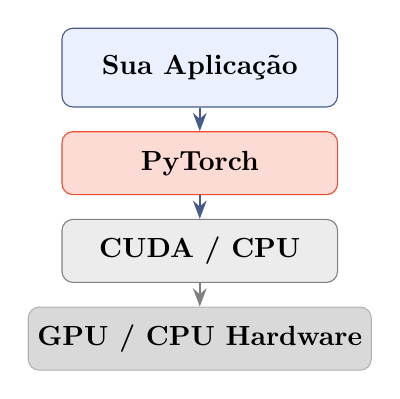
\begin{tikzpicture}
    \node[fill=ptlight, rounded corners, minimum width=3.5cm, minimum height=1cm,
          draw=ptmid] (app) {\textbf{Sua Aplicação}};
    \node[fill=ptred!20, rounded corners, minimum width=3.5cm, minimum height=0.8cm,
          draw=ptred, below=0.3cm of app] (pt) {\textbf{PyTorch}};
    \node[fill=gray!15, rounded corners, minimum width=3.5cm, minimum height=0.8cm,
          draw=gray, below=0.3cm of pt] (cuda) {\textbf{CUDA / CPU}};
    \node[fill=gray!30, rounded corners, minimum width=3.5cm, minimum height=0.8cm,
          draw=gray!60, below=0.3cm of cuda] (hw) {\textbf{GPU / CPU Hardware}};
    \draw[-Stealth, thick, ptmid] (app) -- (pt);
    \draw[-Stealth, thick, ptmid] (pt) -- (cuda);
    \draw[-Stealth, thick, gray] (cuda) -- (hw);
  \end{tikzpicture}
\end{columns}
\end{frame}

% ─────────────────────────────────────────────────────────────────────────────

\begin{frame}{CUDA: CPU vs GPU}
\begin{columns}
\column{0.5\textwidth}
  \begin{block}{CPU}
    \begin{itemize}
      \item 8--32 núcleos otimizados para \textit{latência}
      \item Cache L1/L2/L3 enorme
      \item Bom para tarefas sequenciais
      \item Branches, I/O, lógica complexa
    \end{itemize}
  \end{block}

\column{0.5\textwidth}
  \begin{alertblock}{GPU}
    \begin{itemize}
      \item 4.000--18.000 núcleos CUDA
      \item Otimizada para \textit{throughput}
      \item Ideal para operações matriciais paralelas
      \item RTX 4090: $\approx$ 82 TFLOPS FP32
    \end{itemize}
  \end{alertblock}
\end{columns}

\vspace{0.6em}
\begin{destaque}
  Multiplicar matrizes $1024 \times 1024$: CPU $\approx$ 500ms $\;\longrightarrow\;$ GPU $\approx$ 0.5ms. 
  Fator \textbf{1000$\times$} — e redes neurais são essencialmente multiplicações de matrizes.
\end{destaque}
\end{frame}

% ─────────────────────────────────────────────────────────────────────────────

\begin{frame}[fragile]{Identificando seu CUDA}
\begin{lstlisting}[style=bash]
# Verifica versao do driver CUDA
nvidia-smi

# Saida relevante:
# | CUDA Version: 12.8  |   <- versao do driver
#
# O driver suporta toolkits ate essa versao
# PyTorch eh compilado contra versoes especificas do toolkit
\end{lstlisting}

\vspace{0.5em}
\begin{block}{Versoes de Driver $\times$ Toolkit}
  \centering
  \begin{tabular}{lll}
    \toprule
    Driver CUDA & Toolkit maximo & Wheel PyTorch \\
    \midrule
    $\geq$ 525 & 12.x & \texttt{cu121}, \texttt{cu124} \\
    $\geq$ 550 & 12.4+ & \texttt{cu124} \\
    $\geq$ 570 & 12.8 & \texttt{cu128} \\
    \bottomrule
  \end{tabular}
\end{block}
\end{frame}

% ─────────────────────────────────────────────────────────────────────────────

\begin{frame}[fragile]{Criando o Ambiente e Instalando PyTorch}
\begin{lstlisting}[style=bash]
# 1. Cria ambiente virtual isolado
python -m venv .venv
source .venv/bin/activate          # Linux/macOS
# .venv\Scripts\activate           # Windows

# 2. Instala PyTorch (ajuste cu128 para sua versao de CUDA)
pip install torch torchvision torchaudio \
    --index-url https://download.pytorch.org/whl/cu128

# 3. Verifica instalacao
python -c "
import torch
print('Versao:    ', torch.__version__)
print('CUDA disp.:', torch.cuda.is_available())
print('GPU:       ', torch.cuda.get_device_name(0))
print('Memoria:   ', torch.cuda.get_device_properties(0).total_memory // 1e9, 'GB')
"
\end{lstlisting}

\begin{exampleblock}{Saída esperada}
  \ttfamily\scriptsize
  Versao:     2.5.1+cu128 \\
  CUDA disp.: True \\
  GPU:        NVIDIA GeForce RTX 4090 \\
  Memoria:    24.0 GB
\end{exampleblock}
\end{frame}

% ─────────────────────────────────────────────────────────────────────────────

\begin{frame}[fragile]{Seleção de Device: Padrão de Projeto}
\begin{lstlisting}
import torch

# Padrao recomendado: seleciona automaticamente o melhor device
device = torch.device("cuda" if torch.cuda.is_available() else "cpu")
print(f"Usando: {device}")

# Verificacoes uteis durante o desenvolvimento
print(torch.cuda.device_count())              # numero de GPUs
print(torch.cuda.current_device())           # GPU ativa
torch.cuda.empty_cache()                      # libera cache VRAM
\end{lstlisting}

\vspace{0.4em}
\begin{alertblock}{\faExclamationTriangle\ Regra de Ouro}
  \textbf{Todos} os tensores e o modelo devem estar no \textbf{mesmo device}.
  Misturar CPU e GPU gera erro imediatamente.
\end{alertblock}
\end{frame}

% =============================================================================
\section{Aula 2 — Tensores}
% =============================================================================

\begin{frame}{O que é um Tensor?}
\begin{columns}
\column{0.5\textwidth}
  \begin{block}{Definição Matemática}
    Tensor de ordem $n$: elemento de $\R^{d_1 \times d_2 \times \cdots \times d_n}$
  \end{block}
  \vspace{0.4em}
  \begin{itemize}
    \item \textbf{Ordem 0}: escalar — $3.14$
    \item \textbf{Ordem 1}: vetor — shape $(d)$
    \item \textbf{Ordem 2}: matriz — shape $(m, n)$
    \item \textbf{Ordem 3}: volume — shape $(C, H, W)$
    \item \textbf{Ordem 4}: batch de imagens — shape $(B, C, H, W)$
  \end{itemize}

\column{0.48\textwidth}
  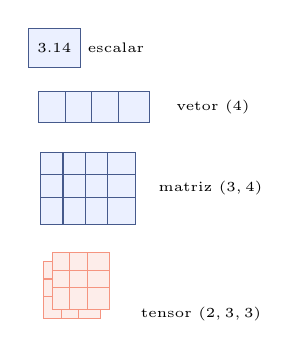
\begin{tikzpicture}[scale=0.75]
    % escalar
    \node[draw=ptmid, fill=ptlight, minimum size=0.5cm] at (0,3) {\tiny 3.14};
    \node[right] at (0.4,3) {\tiny escalar};
    % vetor
    \foreach \i in {0,1,2,3} {
      \node[draw=ptmid, fill=ptlight, minimum size=0.4cm] at (\i*0.45, 2) {};
    }
    \node[right] at (1.9,2) {\tiny vetor $(4)$};
    % matriz
    \foreach \i in {0,1,2} \foreach \j in {0,1,2,3} {
      \node[draw=ptmid, fill=ptlight, minimum size=0.35cm] at (\j*0.38, 1-\i*0.38) {};
    }
    \node[right] at (1.6, 0.62) {\tiny matriz $(3,4)$};
    % tensor 3d
    \foreach \k in {0,1} \foreach \i in {0,1,2} \foreach \j in {0,1,2} {
      \node[draw=ptred!60, fill=ptred!10, minimum size=0.28cm]
        at (\j*0.3 + \k*0.15, -0.8 - \i*0.3 + \k*0.15) {};
    }
    \node[right] at (1.3,-1.5) {\tiny tensor $(2,3,3)$};
  \end{tikzpicture}
\end{columns}
\end{frame}

% ─────────────────────────────────────────────────────────────────────────────

\begin{frame}[fragile]{Criando Tensores}
\begin{columns}
\column{0.5\textwidth}
\begin{lstlisting}
# A partir de dados Python
t = torch.tensor([1.0, 2.0, 3.0])

# Tensores especiais
torch.zeros(3, 4)       # zeros
torch.ones(2, 5)        # uns
torch.eye(4)            # identidade
torch.rand(3, 3)        # uniforme [0,1)
torch.randn(3, 3)       # normal N(0,1)
torch.arange(0, 10, 2)  # [0,2,4,6,8]
torch.linspace(0,1,100) # 100 pontos
\end{lstlisting}

\column{0.48\textwidth}
\begin{lstlisting}
# Inspecionando
x = torch.randn(4, 3, 32, 32)
x.shape       # torch.Size([4,3,32,32])
x.dtype       # torch.float32
x.device      # device(type='cpu')
x.ndim        # 4
x.numel()     # 4*3*32*32 = 12288

# Movendo para GPU
x_gpu = x.to(device)
x_gpu = x.cuda()     # equivalente
x_cpu = x_gpu.cpu()  # de volta
\end{lstlisting}
\end{columns}

\begin{block}{Tipos mais comuns}
  \texttt{float32} (padrão treino) $\cdot$ \texttt{float16} (precisão mista) $\cdot$
  \texttt{int64} (índices) $\cdot$ \texttt{bool} (máscaras)
\end{block}
\end{frame}

% ─────────────────────────────────────────────────────────────────────────────

\begin{frame}[fragile]{Operações Fundamentais}
\begin{columns}
\column{0.5\textwidth}
\begin{lstlisting}
a = torch.tensor([[1.,2.],[3.,4.]])
b = torch.tensor([[5.,6.],[7.,8.]])

# Aritmetica elemento-wise
a + b          # adicao
a * b          # multiplicacao elem.
a ** 2         # potencia

# Algebra linear
a @ b          # multiplicacao matricial
a.T            # transposta
torch.linalg.det(a)   # determinante

# Reducoes
a.sum()        # soma total
a.mean(dim=0)  # media por coluna
a.max()        # maximo
a.argmax()     # indice do maximo
\end{lstlisting}

\column{0.48\textwidth}
\begin{lstlisting}
# Reshape e manipulacao
x = torch.randn(4, 3, 8, 8)
x.view(4, -1)      # (4, 192) -- flat
x.reshape(4, -1)   # igual mas + seguro
x.permute(0,2,3,1) # (4,8,8,3)
x.squeeze()        # remove dims de 1
x.unsqueeze(0)     # adiciona dim

# Indexacao -- igual a NumPy
x[0]               # primeiro do batch
x[:, 0]            # canal 0 de todos
x[0, :, :4, :4]   # recorte espacial

# Concatenacao
torch.cat([a, b], dim=0)   # empilha
torch.stack([a, b], dim=0) # nova dim
\end{lstlisting}
\end{columns}
\end{frame}

% ─────────────────────────────────────────────────────────────────────────────

\begin{frame}[fragile]{Broadcasting — Regra Fundamental}
\begin{block}{Regra}
  Dois tensores são compatíveis se, para cada dimensão (alinhando pela direita), 
  os tamanhos são \textbf{iguais} ou um deles é \textbf{1}.
\end{block}

\begin{lstlisting}
# Exemplo pratico: normalizar batch de imagens
batch  = torch.randn(32, 3, 64, 64)   # (B, C, H, W)
mean   = torch.tensor([0.5, 0.5, 0.5])  # (3,)

# mean precisa de shape (1, 3, 1, 1) para fazer broadcast
batch_norm = batch - mean[None, :, None, None]
#             (32,3,64,64) - (1,3,1,1) -> (32,3,64,64) OK!

# Outro exemplo: adicionar bias a feature maps
feat = torch.randn(8, 128, 16, 16)   # (B, C, H, W)
bias = torch.randn(128)              # (C,)
out  = feat + bias[None, :, None, None]  # broadcast correto
\end{lstlisting}

\begin{alertblock}{\faExclamationTriangle\ Erro comum}
  Esquecer de ajustar as dimensoes antes do broadcast causa
  \texttt{RuntimeError: The size of tensor a (64) must match...}
\end{alertblock}
\end{frame}

% ─────────────────────────────────────────────────────────────────────────────

\begin{frame}[fragile]{In-place vs Out-of-place}
\begin{columns}
\column{0.5\textwidth}
\begin{lstlisting}
x = torch.tensor([1., 2., 3.])

# Out-of-place: cria novo tensor
y = x + 1     # x nao muda
y = x.relu()  # x nao muda

# In-place: modifica o proprio tensor
x.add_(1)         # x = [2, 3, 4]
x.relu_()
x.fill_(0.0)
# operacoes in-place tem sufixo _
\end{lstlisting}

\column{0.48\textwidth}
\begin{alertblock}{Cuidado com in-place e autograd}
  Operações in-place em tensores que fazem parte do grafo 
  computacional \textbf{destroem informações necessárias} para 
  o backward e geram erros.
  \vspace{0.3em}
  
  Regra prática: \textbf{evite} \texttt{\_} em tensores com 
  \texttt{requires\_grad=True}.
\end{alertblock}
\end{columns}

\vspace{0.4em}
\begin{exampleblock}{Numpy $\leftrightarrow$ Tensor (CPU only)}
\begin{lstlisting}[numbers=none]
arr = x.numpy()          # tensor -> numpy (compartilha memoria!)
t   = torch.from_numpy(arr)   # numpy -> tensor
\end{lstlisting}
\end{exampleblock}
\end{frame}

% =============================================================================
\section{Aula 3 — Autograd}
% =============================================================================

\begin{frame}{Diferenciacao Automatica}
\begin{columns}
\column{0.55\textwidth}
  \begin{block}{Ideia Central}
    Cada operacao sobre tensores com \texttt{requires\_grad=True} e registrada 
    num \textbf{grafo computacional}. \texttt{.backward()} percorre esse grafo 
    de tras para frente calculando gradientes pela regra da cadeia.
  \end{block}
  \vspace{0.4em}
  \textbf{Regra da Cadeia:}
  \[
    \frac{dL}{dx} = \frac{dL}{dy} \cdot \frac{dy}{dx}
  \]
  Se $y = f(x)$ e $L = g(y)$:
  \[
    \frac{dL}{dx} = g'(f(x)) \cdot f'(x)
  \]

\column{0.42\textwidth}
  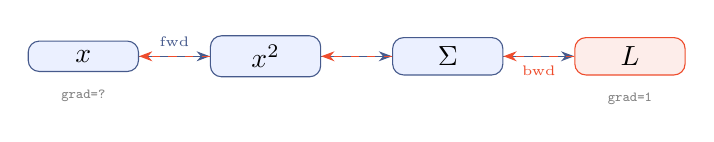
\begin{tikzpicture}[scale=0.85, node distance=0.9cm]
    \node[draw=ptmid, fill=ptlight, rounded corners, minimum width=1.4cm] (x) {$x$};
    \node[draw=ptmid, fill=ptlight, rounded corners, minimum width=1.4cm, right=of x] (sq) {$x^2$};
    \node[draw=ptmid, fill=ptlight, rounded corners, minimum width=1.4cm, right=of sq] (sum) {$\Sigma$};
    \node[draw=ptred, fill=ptred!10, rounded corners, minimum width=1.4cm, right=of sum] (L) {$L$};
    \draw[-Stealth, ptmid] (x) -- node[above]{\tiny fwd} (sq);
    \draw[-Stealth, ptmid] (sq) -- (sum);
    \draw[-Stealth, ptmid] (sum) -- (L);
    \draw[-Stealth, ptred, dashed] (L) -- node[below]{\tiny\color{ptred}bwd} (sum);
    \draw[-Stealth, ptred, dashed] (sum) -- (sq);
    \draw[-Stealth, ptred, dashed] (sq) -- (x);
    \node[below=0.1cm of x, text=cmt] {\tiny \texttt{grad=?}};
    \node[below=0.1cm of L, text=cmt] {\tiny \texttt{grad=1}};
  \end{tikzpicture}
\end{columns}
\end{frame}

% ─────────────────────────────────────────────────────────────────────────────

\begin{frame}[fragile]{Usando o Autograd}
\begin{lstlisting}
import torch

# requires_grad=True: habilita rastreamento de gradientes
x = torch.tensor([2.0, 3.0], requires_grad=True)

# Operacoes sao registradas no grafo
y = x ** 2             # y = [4, 9]
L = y.sum()            # L = 13  (escalar)

# backward() calcula dL/dx para todos os nos do grafo
L.backward()

print(x.grad)
# tensor([4., 6.])   -- correto! dL/dx = 2x

# ATENCAO: gradientes acumulam! Sempre zere antes:
x.grad.zero_()
\end{lstlisting}

\begin{block}{Por que os gradientes acumulam?}
  Por design — útil para gradient accumulation (simular batches maiores).
  Em treino normal, sempre use \texttt{optimizer.zero\_grad()}.
\end{block}
\end{frame}

% ─────────────────────────────────────────────────────────────────────────────

\begin{frame}[fragile]{Desabilitando o Autograd}
\begin{columns}
\column{0.5\textwidth}
\begin{lstlisting}
# Contexto: sem rastreamento
with torch.no_grad():
    pred = model(x_test)
    # operacoes nao vao para o grafo
    # mais rapido, menos memoria

# Decorador para funcoes inteiras
@torch.no_grad()
def avaliar(model, loader):
    for x, y in loader:
        pred = model(x)
        ...
\end{lstlisting}

\column{0.48\textwidth}
\begin{lstlisting}
# .detach(): cria copia sem historico
y = model(x)
y_detached = y.detach()
# y_detached nao propaga gradientes
# util para targets em GANs

# .item(): tensor escalar -> float
loss_val = loss.item()
# IMPORTANTE: usar .item() para logs
# Chamar loss.numpy() nao zera o grafo
\end{lstlisting}
\end{columns}

\begin{destaque}
  \textbf{Regra prática:} use \texttt{torch.no\_grad()} em \textit{qualquer} forward pass 
  fora do treino (validação, inferência, geração). Economiza memória e acelera.
\end{destaque}
\end{frame}

% =============================================================================
\section{Aula 4 — Módulos e Camadas}
% =============================================================================

\begin{frame}[fragile]{O Módulo Base: \texttt{nn.Module}}
\begin{columns}
\column{0.55\textwidth}
\begin{lstlisting}
import torch.nn as nn

class MinhaRede(nn.Module):
    def __init__(self):
        super().__init__()
        # Camadas declaradas aqui
        # sao REGISTRADAS automaticamente
        self.fc1 = nn.Linear(784, 256)
        self.fc2 = nn.Linear(256, 10)

    def forward(self, x):
        # Define o forward pass
        # Backward e calculado automaticamente
        h = torch.relu(self.fc1(x))
        return self.fc2(h)

modelo = MinhaRede()
\end{lstlisting}

\column{0.43\textwidth}
\begin{block}{\texttt{nn.Module} gerencia:}
  \begin{itemize}
    \item Parametros treinaveis\\(\texttt{.parameters()})
    \item Sub-modulos recursivos
    \item Modo treino/avaliacao\\(\texttt{.train()}, \texttt{.eval()})
    \item Serializacao\\(\texttt{.state\_dict()})
    \item Movimentacao de device\\(\texttt{.to(device)})
  \end{itemize}
\end{block}
\end{columns}
\end{frame}

% ─────────────────────────────────────────────────────────────────────────────

\begin{frame}[fragile]{Camadas Essenciais I — Linear e Convolucoes}
\begin{columns}
\column{0.5\textwidth}
\begin{lstlisting}
# Camada totalmente conectada
# y = xW^T + b
nn.Linear(in_features=512,
          out_features=256)

# Convolucao 2D
# (B,C_in,H,W) -> (B,C_out,H',W')
nn.Conv2d(in_channels=3,
          out_channels=64,
          kernel_size=3,
          padding=1,   # preserva HxW
          stride=1)

# Downsampling: stride=2 divide H,W
nn.Conv2d(64, 128, 3, stride=2, padding=1)
# Upsampling: ConvTranspose2D
nn.ConvTranspose2d(128, 64, 4,
                   stride=2, padding=1)
\end{lstlisting}

\column{0.48\textwidth}
  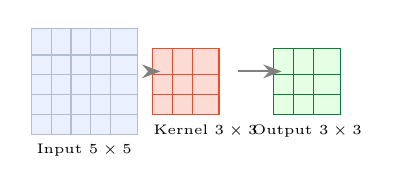
\begin{tikzpicture}[scale=0.7]
    % Input feature map
    \foreach \i in {0,1,2,3,4} \foreach \j in {0,1,2,3,4} {
      \node[draw=ptmid!40, fill=ptlight, minimum size=0.34cm] at (\i*0.36, \j*0.36) {};
    }
    \node[below] at (0.72,-0.25) {\tiny Input $5\times5$};

    % Kernel
    \foreach \i in {0,1,2} \foreach \j in {0,1,2} {
      \node[draw=ptred, fill=ptred!20, minimum size=0.34cm] at (\i*0.36+2.2, \j*0.36+0.36) {};
    }
    \node[below] at (2.92, 0.1) {\tiny Kernel $3\times3$};

    % Output
    \foreach \i in {0,1,2} \foreach \j in {0,1,2} {
      \node[draw=str, fill=green!10, minimum size=0.34cm] at (\i*0.36+4.4, \j*0.36+0.36) {};
    }
    \node[below] at (4.76, 0.1) {\tiny Output $3\times3$};

    \draw[-Stealth, thick, gray] (1.9,0.9) -- (2.1,0.9);
    \draw[-Stealth, thick, gray] (3.5,0.9) -- (4.3,0.9);
  \end{tikzpicture}
  \vspace{0.3em}
  \[\text{out\_size} = \left\lfloor\frac{H + 2p - k}{s}\right\rfloor + 1\]
\end{columns}
\end{frame}

% ─────────────────────────────────────────────────────────────────────────────

\begin{frame}[fragile]{Camadas Essenciais II — Normalização}
\begin{columns}
\column{0.5\textwidth}
\begin{lstlisting}
# BatchNorm: normaliza por batch
# Bom para batches grandes (>= 32)
nn.BatchNorm2d(num_features=64)

# GroupNorm: normaliza por grupo de canais
# Funciona com batch size pequeno
# Preferido em score matching e difusao
nn.GroupNorm(num_groups=8,
             num_channels=64)
# Regra: num_channels % num_groups == 0

# LayerNorm: normaliza por token (Transformers)
nn.LayerNorm(normalized_shape=512)

# InstanceNorm: normaliza por imagem
# Comum em style transfer
nn.InstanceNorm2d(num_features=64)
\end{lstlisting}

\column{0.48\textwidth}
\begin{block}{Formula Geral de Normalizacao}
  \[\hat{x} = \frac{x - \mu}{\sqrt{\sigma^2 + \epsilon}} \cdot \gamma + \beta\]
  $\gamma, \beta$: parametros aprendiveis\\
  $\epsilon$: estabilidade numerica ($10^{-5}$)
\end{block}
\vspace{0.3em}
\begin{block}{Diferenca entre elas}
  \centering
  \begin{tabular}{lc}
    \toprule
    Tipo & Normaliza sobre \\
    \midrule
    BatchNorm & batch + HW \\
    GroupNorm & grupos de C \\
    LayerNorm & toda a feature \\
    InstanceNorm & H + W \\
    \bottomrule
  \end{tabular}
\end{block}
\end{columns}
\end{frame}

% ─────────────────────────────────────────────────────────────────────────────

\begin{frame}[fragile]{Camadas Essenciais III — Ativacoes e Pooling}
\begin{columns}
\column{0.5\textwidth}
\begin{lstlisting}
# Ativacoes comuns
nn.ReLU()              # max(0, x)
nn.LeakyReLU(0.2)      # usado em GANs
nn.SiLU()              # x * sigmoid(x)
nn.GELU()              # padrao Transformers
nn.Tanh()              # [-1, 1] -- GANs output
nn.Sigmoid()           # [0, 1]
nn.Softmax(dim=-1)     # soma 1 -- classificacao

# Pooling
nn.MaxPool2d(kernel_size=2, stride=2)
nn.AvgPool2d(kernel_size=2, stride=2)
nn.AdaptiveAvgPool2d((1, 1))  # global avg

# Dropout
nn.Dropout(p=0.5)       # para vetores
nn.Dropout2d(p=0.5)     # para feature maps
\end{lstlisting}

\column{0.48\textwidth}
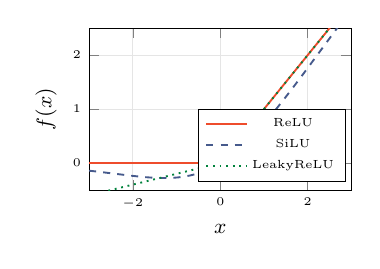
\begin{tikzpicture}[scale=0.85]
\begin{axis}[
  width=5.5cm, height=4cm,
  xlabel={\small $x$}, ylabel={\small $f(x)$},
  xmin=-3, xmax=3, ymin=-0.5, ymax=2.5,
  legend style={font=\tiny, at={(0.98,0.05)}, anchor=south east},
  grid=major, grid style={gray!20},
  tick label style={font=\tiny},
  label style={font=\small},
]
\addplot[ptred, thick, domain=-3:3, samples=60] {max(0,x)};
\addlegendentry{ReLU}
\addplot[ptmid, thick, dashed, domain=-3:3, samples=60] {x/(1+exp(-x))};
\addlegendentry{SiLU}
\addplot[str, thick, dotted, domain=-3:3, samples=60] {max(0.2*x, x)};
\addlegendentry{LeakyReLU}
\end{axis}
\end{tikzpicture}
\end{columns}
\end{frame}

% ─────────────────────────────────────────────────────────────────────────────

\begin{frame}[fragile]{Compondo Módulos: \texttt{nn.Sequential}}
\begin{columns}
\column{0.5\textwidth}
\begin{lstlisting}
# Sequential: pilha ordenada de camadas
bloco_conv = nn.Sequential(
    nn.Conv2d(3, 64, 3, padding=1),
    nn.BatchNorm2d(64),
    nn.ReLU(),
    nn.Conv2d(64, 64, 3, padding=1),
    nn.BatchNorm2d(64),
    nn.ReLU(),
    nn.MaxPool2d(2, 2),
)

# ModuleList: lista de modulos
self.camadas = nn.ModuleList([
    nn.Linear(512, 256),
    nn.Linear(256, 128),
    nn.Linear(128, 64),
])

# ModuleDict: dicionario de modulos
self.heads = nn.ModuleDict({
    'classificacao': nn.Linear(64, 10),
    'regressao': nn.Linear(64, 1),
})
\end{lstlisting}

\column{0.48\textwidth}
\begin{alertblock}{NUNCA use lista Python pura!}
\begin{lstlisting}[numbers=none]
# ERRADO -- PyTorch nao vê
self.layers = [
    nn.Linear(128,64),
    nn.Linear(64, 32),
]
# parametros NAO serao treinados!

# CERTO
self.layers = nn.ModuleList([
    nn.Linear(128, 64),
    nn.Linear(64, 32),
])
\end{lstlisting}
\end{alertblock}
\end{columns}
\end{frame}

% ─────────────────────────────────────────────────────────────────────────────

\begin{frame}[fragile]{Inspecao do Modelo}
\begin{lstlisting}
model = MinhaRede().to(device)

# Conta parametros
total  = sum(p.numel() for p in model.parameters())
treina = sum(p.numel() for p in model.parameters() if p.requires_grad)
print(f"Total: {total:,}  |  Treinaveis: {treina:,}")

# state_dict: dicionario nome -> tensor dos parametros
for nome, param in model.state_dict().items():
    print(f"{nome:30s}  {str(param.shape):25s}  {param.numel():>8,}")

# Modo treino vs avaliacao
model.train()   # ativa Dropout e BatchNorm em modo treino
model.eval()    # desativa Dropout, BatchNorm usa media movel

# Congelar parametros (ex: transfer learning)
for param in model.fc1.parameters():
    param.requires_grad = False
\end{lstlisting}
\end{frame}

% =============================================================================
\section{Aula 5 — Dados: Dataset e DataLoader}
% =============================================================================

\begin{frame}[fragile]{A Abstração de Dados}
\begin{columns}
\column{0.5\textwidth}
\begin{block}{Dataset}
  Encapsula \textbf{de onde} vêm os dados.\\
  Dois métodos obrigatórios:
  \begin{itemize}
    \item \texttt{\_\_len\_\_}: tamanho total
    \item \texttt{\_\_getitem\_\_}: um item pelo índice
  \end{itemize}
\end{block}
\vspace{0.3em}
\begin{block}{DataLoader}
  Encapsula \textbf{como} os dados chegam:
  \begin{itemize}
    \item Batching automático
    \item Shuffling
    \item Paralelismo (\texttt{num\_workers})
    \item Prefetching
  \end{itemize}
\end{block}

\column{0.48\textwidth}
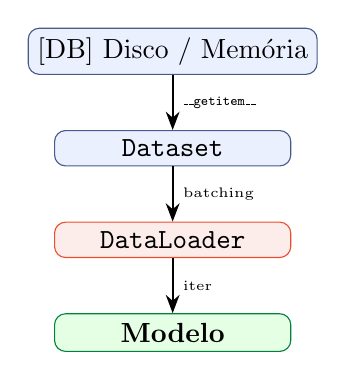
\begin{tikzpicture}[node distance=0.7cm, scale=0.9]
  \node[draw=ptmid, fill=ptlight, rounded corners, minimum width=3cm, text centered]
    (disk) {\faDatabase\ Disco / Memória};
  \node[draw=ptmid, fill=ptlight, rounded corners, minimum width=3cm, text centered,
        below=of disk]
    (ds) {\texttt{Dataset}};
  \node[draw=ptred, fill=ptred!10, rounded corners, minimum width=3cm, text centered,
        below=of ds]
    (dl) {\texttt{DataLoader}};
  \node[draw=str, fill=green!10, rounded corners, minimum width=3cm, text centered,
        below=of dl]
    (model) {\textbf{Modelo}};
  \draw[-Stealth, thick] (disk) -- (ds) node[midway, right]{\tiny \texttt{\_\_getitem\_\_}};
  \draw[-Stealth, thick] (ds) -- (dl) node[midway, right]{\tiny batching};
  \draw[-Stealth, thick] (dl) -- (model) node[midway, right]{\tiny iter};
\end{tikzpicture}
\end{columns}
\end{frame}

% ─────────────────────────────────────────────────────────────────────────────

\begin{frame}[fragile]{Criando um Dataset Customizado}
\begin{lstlisting}
from torch.utils.data import Dataset, DataLoader

class MeuDataset(Dataset):
    def __init__(self, imagens, rotulos, transform=None):
        # imagens: tensor (N, C, H, W) ou lista de paths
        self.imagens  = imagens
        self.rotulos  = rotulos
        self.transform = transform

    def __len__(self):
        return len(self.imagens)   # tamanho total do dataset

    def __getitem__(self, idx):
        x = self.imagens[idx]      # uma amostra
        y = self.rotulos[idx]      # seu rotulo

        if self.transform:
            x = self.transform(x)

        return x, y

# Instancia e encapsula no DataLoader
dataset = MeuDataset(X_train, y_train)
loader  = DataLoader(dataset, batch_size=64, shuffle=True, num_workers=4)
\end{lstlisting}
\end{frame}

% ─────────────────────────────────────────────────────────────────────────────

\begin{frame}[fragile]{Usando o DataLoader}
\begin{lstlisting}
# Iteracao padrao sobre um DataLoader
for x_batch, y_batch in loader:
    # x_batch: (batch_size, C, H, W)
    # y_batch: (batch_size,)
    x_batch = x_batch.to(device)
    y_batch = y_batch.to(device)
    # ... treino ...

# Datasets prontos do torchvision
import torchvision
import torchvision.transforms as T

transform = T.Compose([
    T.ToTensor(),              # PIL/numpy -> tensor [0,1]
    T.Normalize((0.5,), (0.5,)),  # normaliza para [-1,1]
    T.RandomHorizontalFlip(),  # augmentacao
])

mnist = torchvision.datasets.MNIST(
    root='./data', train=True, download=True, transform=transform
)
loader = DataLoader(mnist, batch_size=128, shuffle=True, num_workers=4)
\end{lstlisting}
\end{frame}

% =============================================================================
\section{Aula 6 — Funções de Perda e Otimizadores}
% =============================================================================

\begin{frame}{Funções de Perda}
\begin{columns}
\column{0.5\textwidth}
\begin{block}{Classificação}
  \textbf{CrossEntropyLoss:}
  \[ L = -\sum_c y_c \log \hat{p}_c \]
  Combina LogSoftmax + NLLLoss.
  
  \vspace{0.3em}
  \textbf{BCEWithLogitsLoss:}
  \[ L = -[y\log\sigma(x) + (1-y)\log(1-\sigma(x))] \]
  Para classificação binária (GANs!).
\end{block}

\column{0.48\textwidth}
\begin{block}{Regressão}
  \textbf{MSELoss:}
  \[ L = \frac{1}{N}\sum (y_i - \hat{y}_i)^2 \]
  
  \textbf{L1Loss (MAE):}
  \[ L = \frac{1}{N}\sum |y_i - \hat{y}_i| \]
  
  \textbf{HuberLoss:} combinação robusta de L1+L2
\end{block}
\end{columns}
\end{frame}

% ─────────────────────────────────────────────────────────────────────────────

\begin{frame}[fragile]{Usando Funções de Perda}
\begin{lstlisting}
import torch.nn as nn

# CrossEntropy: logits (antes do softmax) vs indices de classe
criterio = nn.CrossEntropyLoss()
logits   = torch.randn(32, 10)   # (batch, num_classes)
rotulos  = torch.randint(0, 10, (32,))  # indices [0..9]
loss = criterio(logits, rotulos)

# BCEWithLogits: logits vs probabilidades alvo (GANs)
criterio_bce = nn.BCEWithLogitsLoss()
pred   = torch.randn(32, 1)       # discriminador
real   = torch.ones(32, 1)        # label "real" = 1
falso  = torch.zeros(32, 1)       # label "falso" = 0
loss_real  = criterio_bce(pred, real)
loss_falso = criterio_bce(pred, falso)

# MSE: para regressao e reconstrucao
criterio_mse = nn.MSELoss()
pred_reg = torch.randn(32, 1)
alvo_reg = torch.randn(32, 1)
loss_reg = criterio_mse(pred_reg, alvo_reg)
\end{lstlisting}
\end{frame}

% ─────────────────────────────────────────────────────────────────────────────

\begin{frame}{Otimizadores: Como os Parametros Atualizam}
\begin{block}{Regra Geral de Atualizacao}
  \[ \theta_{t+1} = \theta_t - \alpha \cdot v_t \]
  onde $v_t$ e a \textbf{direcao} de atualizacao (depende do otimizador).
\end{block}

\vspace{0.4em}
\begin{columns}
\column{0.5\textwidth}
\begin{block}{SGD com Momentum}
  \[ v_t = \beta v_{t-1} + \nabla L(\theta_t) \]
  \[ \theta_{t+1} = \theta_t - \alpha v_t \]
  Acumula gradientes anteriores. Robusto, requer tuning de $\alpha$.
\end{block}

\column{0.48\textwidth}
\begin{block}{Adam}
  \[ m_t = \beta_1 m_{t-1} + (1-\beta_1)\nabla L \]
  \[ v_t = \beta_2 v_{t-1} + (1-\beta_2)(\nabla L)^2 \]
  \[ \theta \leftarrow \theta - \frac{\alpha}{\sqrt{\hat{v}_t} + \epsilon}\hat{m}_t \]
  Step adaptativo por parametro. Padrao para deep learning.
\end{block}
\end{columns}
\end{frame}

% ─────────────────────────────────────────────────────────────────────────────

\begin{frame}[fragile]{Usando Otimizadores}
\begin{lstlisting}
import torch.optim as optim

model = MinhaRede().to(device)

# Adam: padrao para a maioria dos casos
optimizer = optim.Adam(model.parameters(), lr=1e-3, weight_decay=1e-4)

# SGD com momentum: bom para CNNs supervisionadas
optimizer = optim.SGD(model.parameters(), lr=0.01, momentum=0.9)

# AdamW: Adam com weight decay correto (preferido em Transformers)
optimizer = optim.AdamW(model.parameters(), lr=1e-4, weight_decay=0.01)

# Diferentes learning rates por modulo
optimizer = optim.Adam([
    {'params': model.encoder.parameters(), 'lr': 1e-4},
    {'params': model.decoder.parameters(), 'lr': 1e-3},
])

# Learning rate scheduling
scheduler = optim.lr_scheduler.CosineAnnealingLR(optimizer, T_max=100)
scheduler = optim.lr_scheduler.StepLR(optimizer, step_size=30, gamma=0.1)
\end{lstlisting}
\end{frame}

% =============================================================================
\section{Aula 7 — O Loop de Treinamento}
% =============================================================================

\begin{frame}[fragile]{O Loop Completo}
\begin{lstlisting}[style=small]
def treinar(model, train_loader, val_loader, n_epochs=50, lr=1e-3):
    model = model.to(device)
    optimizer = optim.Adam(model.parameters(), lr=lr)
    criterio  = nn.CrossEntropyLoss()

    for epoch in range(n_epochs):
        # ── FASE DE TREINO ──────────────────────────────────────────
        model.train()
        loss_treino = 0.0
        for x, y in train_loader:
            x, y = x.to(device), y.to(device)

            pred = model(x)                    # 1. Forward
            loss = criterio(pred, y)           # 2. Calcula loss

            optimizer.zero_grad()              # 3. Zera gradientes
            loss.backward()                    # 4. Backward (gradientes)
            optimizer.step()                   # 5. Atualiza parametros

            loss_treino += loss.item()

        # ── FASE DE VALIDACAO ───────────────────────────────────────
        model.eval()
        loss_val, acertos = 0.0, 0
        with torch.no_grad():
            for x, y in val_loader:
                x, y = x.to(device), y.to(device)
                pred = model(x)
                loss_val += criterio(pred, y).item()
                acertos  += (pred.argmax(1) == y).sum().item()

        acc = acertos / len(val_loader.dataset)
        print(f"Epoca {epoch+1:3d} | Loss treino: {loss_treino/len(train_loader):.4f} "
              f"| Loss val: {loss_val/len(val_loader):.4f} | Acc: {acc:.3f}")
\end{lstlisting}
\end{frame}

% ─────────────────────────────────────────────────────────────────────────────

\begin{frame}{Os 5 Passos do Loop — Mapa Mental}
\begin{center}
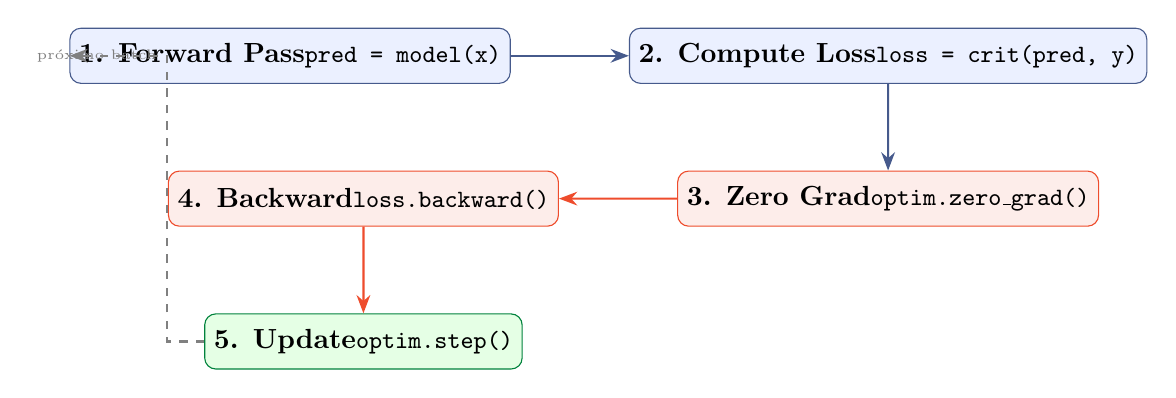
\begin{tikzpicture}[node distance=1.1cm, scale=0.95]
  \node[draw=ptmid, fill=ptlight, rounded corners, minimum width=3cm, minimum height=0.7cm,
        text centered] (fwd) {\textbf{1. Forward Pass}\\\small\texttt{pred = model(x)}};
  \node[draw=ptmid, fill=ptlight, rounded corners, minimum width=3cm, minimum height=0.7cm,
        text centered, right=1.5cm of fwd] (loss) {\textbf{2. Compute Loss}\\\small\texttt{loss = crit(pred, y)}};
  \node[draw=ptred, fill=ptred!10, rounded corners, minimum width=3cm, minimum height=0.7cm,
        text centered, below=of loss] (zero) {\textbf{3. Zero Grad}\\\small\texttt{optim.zero\_grad()}};
  \node[draw=ptred, fill=ptred!10, rounded corners, minimum width=3cm, minimum height=0.7cm,
        text centered, left=1.5cm of zero] (bwd) {\textbf{4. Backward}\\\small\texttt{loss.backward()}};
  \node[draw=str, fill=green!10, rounded corners, minimum width=3cm, minimum height=0.7cm,
        text centered, below=of bwd] (step) {\textbf{5. Update}\\\small\texttt{optim.step()}};

  \draw[-Stealth, thick, ptmid] (fwd) -- (loss);
  \draw[-Stealth, thick, ptmid] (loss) -- (zero);
  \draw[-Stealth, thick, ptred] (zero) -- (bwd);
  \draw[-Stealth, thick, ptred] (bwd) -- (step);
  \draw[-Stealth, thick, gray, dashed] (step.west) -- ++(-0.5,0) |- (fwd.west)
    node[midway, left, font=\tiny] {próximo batch};
\end{tikzpicture}
\end{center}

\begin{alertblock}{Ordem importa!}
  \textbf{zero\_grad()} deve vir \textit{antes} do \texttt{backward()}.
  Caso contrário, gradientes acumulam sobre os passos anteriores.
\end{alertblock}
\end{frame}

% ─────────────────────────────────────────────────────────────────────────────

\begin{frame}[fragile]{Salvando e Carregando Modelos}
\begin{lstlisting}
# ── SALVAR ──────────────────────────────────────────────────────────────
# Recomendado: salva apenas os pesos (state_dict)
torch.save(model.state_dict(), 'modelo.pth')

# Checkpoint completo (para retomar treino)
torch.save({
    'epoch':      epoch,
    'model':      model.state_dict(),
    'optimizer':  optimizer.state_dict(),
    'loss':       best_loss,
}, 'checkpoint.pth')

# ── CARREGAR ─────────────────────────────────────────────────────────────
# Carregar pesos
model = MinhaRede()
model.load_state_dict(torch.load('modelo.pth', map_location=device))
model.eval()

# Retomar treino a partir do checkpoint
checkpoint = torch.load('checkpoint.pth')
model.load_state_dict(checkpoint['model'])
optimizer.load_state_dict(checkpoint['optimizer'])
epoch_inicio = checkpoint['epoch']
\end{lstlisting}
\end{frame}

% =============================================================================
\section{Aula 8 — Padrões de Arquitetura}
% =============================================================================

\begin{frame}[fragile]{Bloco Residual (ResBlock)}
\begin{columns}
\column{0.5\textwidth}
\begin{block}{Ideia (He et al. 2015)}
  Em vez de aprender $H(x)$, aprende a \textbf{resíduo} $F(x) = H(x) - x$:
  \[ y = F(x) + x \]
  Isso facilita treinar redes muito profundas — o gradiente flui diretamente pela skip connection.
\end{block}

\begin{lstlisting}[basicstyle=\ttfamily\tiny]
class ResBlock(nn.Module):
    def __init__(self, channels):
        super().__init__()
        self.bloco = nn.Sequential(
            nn.Conv2d(channels, channels, 3, padding=1),
            nn.BatchNorm2d(channels),
            nn.ReLU(),
            nn.Conv2d(channels, channels, 3, padding=1),
            nn.BatchNorm2d(channels),
        )
    def forward(self, x):
        return torch.relu(self.bloco(x) + x)
\end{lstlisting}

\column{0.45\textwidth}
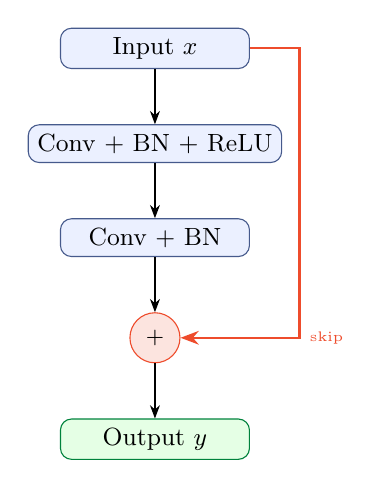
\begin{tikzpicture}[scale=0.9, node distance=0.7cm]
  \node[draw=ptmid, fill=ptlight, rounded corners, minimum width=2.4cm,
        text centered, font=\small] (inp) {Input $x$};
  \node[draw=ptmid, fill=ptlight, rounded corners, minimum width=2.4cm,
        text centered, font=\small, below=of inp] (conv1) {Conv + BN + ReLU};
  \node[draw=ptmid, fill=ptlight, rounded corners, minimum width=2.4cm,
        text centered, font=\small, below=of conv1] (conv2) {Conv + BN};
  \node[draw=ptred, fill=ptred!15, circle, minimum size=0.6cm,
        text centered, font=\footnotesize, below=of conv2] (add) {$+$};
  \node[draw=str, fill=green!10, rounded corners, minimum width=2.4cm,
        text centered, font=\small, below=of add] (out) {Output $y$};
  \draw[-Stealth] (inp) -- (conv1);
  \draw[-Stealth] (conv1) -- (conv2);
  \draw[-Stealth] (conv2) -- (add);
  \draw[-Stealth] (add) -- (out);
  % skip connection
  \draw[-Stealth, ptred, thick] (inp.east) -- ++(0.7,0) |- (add.east)
    node[midway, right, font=\tiny] {skip};
\end{tikzpicture}
\end{columns}
\end{frame}

% ─────────────────────────────────────────────────────────────────────────────

\begin{frame}[fragile]{Encoder-Decoder e U-Net}
\begin{columns}
\column{0.52\textwidth}
\begin{lstlisting}[style=small]
class UNet(nn.Module):
    def __init__(self, in_ch=1, out_ch=1):
        super().__init__()
        # Encoder: reduz espacialmente
        self.enc1 = self._bloco(in_ch, 64)
        self.enc2 = self._bloco(64, 128)
        self.enc3 = self._bloco(128, 256)
        self.pool = nn.MaxPool2d(2)

        # Bottleneck
        self.mid = self._bloco(256, 512)

        # Decoder: expande + skip connections
        self.up3 = nn.ConvTranspose2d(512,256,2,stride=2)
        self.dec3 = self._bloco(512, 256) # 256+256 skip
        self.up2 = nn.ConvTranspose2d(256,128,2,stride=2)
        self.dec2 = self._bloco(256, 128)
        self.up1 = nn.ConvTranspose2d(128, 64,2,stride=2)
        self.dec1 = self._bloco(128, 64)

        self.out = nn.Conv2d(64, out_ch, 1)

    def _bloco(self, c_in, c_out):
        return nn.Sequential(
            nn.Conv2d(c_in, c_out, 3, padding=1),
            nn.BatchNorm2d(c_out), nn.ReLU(),
            nn.Conv2d(c_out, c_out, 3, padding=1),
            nn.BatchNorm2d(c_out), nn.ReLU(),
        )

    def forward(self, x):
        e1 = self.enc1(x)
        e2 = self.enc2(self.pool(e1))
        e3 = self.enc3(self.pool(e2))
        m  = self.mid(self.pool(e3))
        d3 = self.dec3(torch.cat([self.up3(m), e3], 1))
        d2 = self.dec2(torch.cat([self.up2(d3),e2], 1))
        d1 = self.dec1(torch.cat([self.up1(d2),e1], 1))
        return self.out(d1)
\end{lstlisting}

\column{0.46\textwidth}
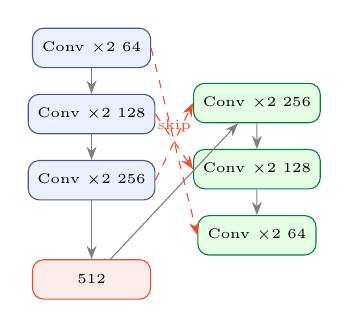
\begin{tikzpicture}[scale=0.7, node distance=0.5cm]
  % Encoder
  \foreach \i/\c in {0/64, 1/128, 2/256} {
    \node[draw=ptmid, fill=ptlight, rounded corners, minimum width=1.5cm,
          minimum height=0.5cm, text centered, font=\tiny] (e\i) at (0, -\i*1.2) {Conv $\times2$ \c};
  }
  % Bottleneck
  \node[draw=ptred, fill=ptred!10, rounded corners, minimum width=1.5cm,
        minimum height=0.5cm, text centered, font=\tiny] (mid) at (0, -4.2) {512};
  % Decoder
  \foreach \i/\c in {0/256, 1/128, 2/64} {
    \node[draw=str, fill=green!10, rounded corners, minimum width=1.5cm,
          minimum height=0.5cm, text centered, font=\tiny] (d\i) at (3, -\i*1.2-1.0) {Conv $\times2$ \c};
  }
  % Arrows down
  \draw[-Stealth, gray] (e0) -- (e1);
  \draw[-Stealth, gray] (e1) -- (e2);
  \draw[-Stealth, gray] (e2) -- (mid);
  % Arrows up
  \draw[-Stealth, gray] (mid) -- (d0);
  \draw[-Stealth, gray] (d0) -- (d1);
  \draw[-Stealth, gray] (d1) -- (d2);
  % Skip connections
  \draw[-Stealth, ptred, dashed] (e2.east) -- (d0.west) node[midway, above, font=\tiny]{skip};
  \draw[-Stealth, ptred, dashed] (e1.east) -- (d1.west);
  \draw[-Stealth, ptred, dashed] (e0.east) -- (d2.west);
\end{tikzpicture}
\end{columns}
\end{frame}

% =============================================================================
\section{Aula 9 — Perceptron}
% =============================================================================

\begin{frame}{O Neuronio Artificial}
\begin{columns}
\column{0.52\textwidth}
  \begin{block}{Modelo de McCulloch-Pitts (1943)}
    O neuronio artificial recebe $n$ entradas, calcula uma soma ponderada e aplica 
    uma funcao de ativacao:
    \[
      y = f\!\left(\sum_{i=1}^n w_i x_i + b\right) = f(\mathbf{w}^\top \mathbf{x} + b)
    \]
    Parametros aprendidos: \textbf{pesos} $\mathbf{w}$ e \textbf{bias} $b$.
  \end{block}
  \vspace{0.3em}
  \begin{itemize}
    \item Perceptron (Rosenblatt, 1958): $f = $ step function
    \item Aprende com regra de Hebb: $w \leftarrow w + \eta (y - \hat{y}) x$
    \item Limitacao: so classifica problemas \textbf{linearmente separaveis}
  \end{itemize}

\column{0.45\textwidth}
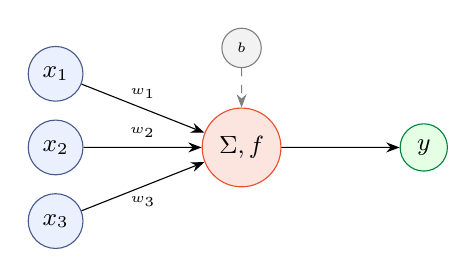
\begin{tikzpicture}[scale=0.85, node distance=0.8cm]
  % Inputs
  \foreach \i/\v in {1/$x_1$, 2/$x_2$, 3/$x_3$} {
    \node[draw=ptmid, fill=ptlight, circle, minimum size=0.6cm, font=\small]
      (x\i) at (0, -\i*1.1+1.7) {\v};
  }
  % Neuron
  \node[draw=ptred, fill=ptred!15, circle, minimum size=1cm,
        font=\small, right=1.5cm of x2] (n) {$\Sigma, f$};
  % Output
  \node[draw=str, fill=green!10, circle, minimum size=0.6cm,
        font=\small, right=1.5cm of n] (out) {$y$};
  % Edges with weights
  \draw[-Stealth] (x1) -- node[above, font=\tiny]{$w_1$} (n);
  \draw[-Stealth] (x2) -- node[above, font=\tiny]{$w_2$} (n);
  \draw[-Stealth] (x3) -- node[below, font=\tiny]{$w_3$} (n);
  \draw[-Stealth] (n) -- (out);
  % Bias
  \node[draw=gray, fill=gray!10, circle, minimum size=0.5cm,
        font=\tiny, above=0.5cm of n] (b) {$b$};
  \draw[-Stealth, dashed, gray] (b) -- (n);
\end{tikzpicture}
\end{columns}
\end{frame}

% ─────────────────────────────────────────────────────────────────────────────

\begin{frame}[fragile]{Perceptron em PyTorch}
\begin{columns}
\column{0.5\textwidth}
\begin{lstlisting}
import torch
import torch.nn as nn

# Um unico neuronio = nn.Linear(in, 1)
# para classificacao binaria
class Perceptron(nn.Module):
    def __init__(self, n_entradas: int):
        super().__init__()
        # w: (n_entradas,), b: escalar
        self.linear = nn.Linear(n_entradas, 1)

    def forward(self, x: torch.Tensor):
        # x: (B, n_entradas)
        logit = self.linear(x)  # (B, 1)
        return logit             # sem sigmoid
                                 # BCEWithLogitsLoss

# Treino
modelo = Perceptron(n_entradas=2)
opt    = torch.optim.SGD(
             modelo.parameters(), lr=0.1)
crit   = nn.BCEWithLogitsLoss()
\end{lstlisting}

\column{0.48\textwidth}
\begin{lstlisting}
# Gerando dataset linearmente separavel
# XOR nao funcionaria com um Perceptron!
X = torch.tensor([
    [0., 0.], [0., 1.],
    [1., 0.], [1., 1.],
])
y = torch.tensor([[0.],[0.],[0.],[1.]])  # AND

# Loop simples
for epoch in range(300):
    pred = modelo(X)
    loss = crit(pred, y)
    opt.zero_grad()
    loss.backward()
    opt.step()

# Resultado
with torch.no_grad():
    prob = torch.sigmoid(modelo(X))
    print(prob.round())
    # tensor([[0.],[0.],[0.],[1.]])
\end{lstlisting}
\end{columns}
\end{frame}

% ─────────────────────────────────────────────────────────────────────────────

\begin{frame}{Limitacao do Perceptron: XOR}
\begin{columns}
\column{0.5\textwidth}
\begin{block}{Problema XOR}
  O Perceptron nao consegue aprender XOR porque XOR nao e 
  \textbf{linearmente separavel}: nao existe uma linha reta que 
  divida as classes.

  \begin{center}
  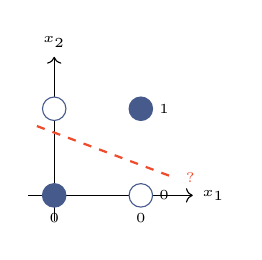
\begin{tikzpicture}[scale=1.1]
    \draw[->] (-0.3,0) -- (1.6,0) node[right]{\tiny $x_1$};
    \draw[->] (0,-0.3) -- (0,1.6) node[above]{\tiny $x_2$};
    % Pontos XOR
    \node[draw=ptmid, fill=ptmid, circle, inner sep=3pt] at (0,0) {};
    \node[draw=ptmid, fill=white,  circle, inner sep=3pt] at (0,1) {};
    \node[draw=ptmid, fill=white,  circle, inner sep=3pt] at (1,0) {};
    \node[draw=ptmid, fill=ptmid, circle, inner sep=3pt] at (1,1) {};
    \node[right, font=\tiny] at (1.1,0)  {0};
    \node[right, font=\tiny] at (1.1,1)  {1};
    \node[below, font=\tiny] at (0,-0.1) {0};
    \node[below, font=\tiny] at (1,-0.1) {0};
    % Tentativa de separacao (falha)
    \draw[ptred, dashed, thick] (-0.2, 0.8) -- (1.4, 0.2)
      node[right, font=\tiny, ptred]{?};
  \end{tikzpicture}
  \end{center}
\end{block}

\column{0.48\textwidth}
\begin{alertblock}{Solucao: empilhar neuronios}
  Um unico neuronio so aprende fronteiras lineares.\\
  \vspace{0.4em}
  Para aprender XOR e necessario \textbf{pelo menos uma camada oculta} 
  com funcoes de ativacao nao-lineares --- esse e o MLP.\\
  \vspace{0.4em}
  Teorema da Aproximacao Universal: um MLP com uma camada oculta 
  suficientemente grande pode aproximar \textbf{qualquer funcao continua}.
\end{alertblock}
\end{columns}
\end{frame}

% =============================================================================
\section{Aula 10 — MLP}
% =============================================================================

\begin{frame}{Multi-Layer Perceptron}
\begin{columns}
\column{0.5\textwidth}
  \begin{block}{Definicao}
    MLP e uma rede com pelo menos uma \textbf{camada oculta} entre 
    entrada e saida. Cada camada aplica:
    \[
      \mathbf{h}^{(l)} = f\!\left(W^{(l)}\mathbf{h}^{(l-1)} + \mathbf{b}^{(l)}\right)
    \]
    A nao-linearidade $f$ e essencial --- sem ela, empilhar camadas 
    seria equivalente a uma unica transformacao linear.
  \end{block}
  \vspace{0.3em}
  \textbf{Por que funciona?}\\
  Cada camada aprende uma \emph{representacao} mais abstrata da entrada. 
  Pixels $\to$ bordas $\to$ formas $\to$ conceitos.

\column{0.48\textwidth}
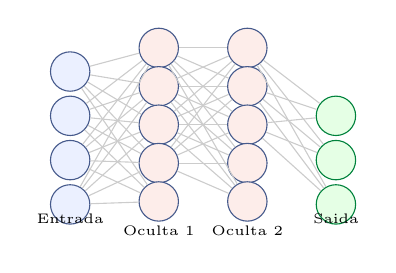
\begin{tikzpicture}[scale=0.75, node distance=0.5cm]
  % Input layer
  \foreach \i in {1,2,3,4} {
    \node[draw=ptmid, fill=ptlight, circle, minimum size=0.5cm]
      (i\i) at (0, -\i*0.75+1.5) {};
  }
  \node[below, font=\tiny] at (0, -1.5) {Entrada};
  % Hidden layer 1
  \foreach \i in {1,2,3,4,5} {
    \node[draw=ptmid, fill=ptred!10, circle, minimum size=0.5cm]
      (h1\i) at (1.5, -\i*0.65+1.8) {};
  }
  \node[below, font=\tiny] at (1.5, -1.7) {Oculta 1};
  % Hidden layer 2
  \foreach \i in {1,2,3,4,5} {
    \node[draw=ptmid, fill=ptred!10, circle, minimum size=0.5cm]
      (h2\i) at (3.0, -\i*0.65+1.8) {};
  }
  \node[below, font=\tiny] at (3.0, -1.7) {Oculta 2};
  % Output
  \foreach \i in {1,2,3} {
    \node[draw=str, fill=green!10, circle, minimum size=0.5cm]
      (o\i) at (4.5, -\i*0.75+0.75) {};
  }
  \node[below, font=\tiny] at (4.5, -1.5) {Saida};
  % Edges (sample)
  \foreach \i in {1,2,3,4} \foreach \j in {1,2,3,4,5} {
    \draw[gray!40, thin] (i\i) -- (h1\j);
    \draw[gray!40, thin] (h1\i) -- (h2\j);
  }
  \foreach \i in {1,2,3} \foreach \j in {1,2,3} {
    \draw[gray!40, thin] (h2\i) -- (o\j);
  }
\end{tikzpicture}
\end{columns}
\end{frame}

% ─────────────────────────────────────────────────────────────────────────────

\begin{frame}[fragile]{Implementando um MLP}
\begin{lstlisting}
class MLP(nn.Module):
    """
    MLP generico e configuravel.
    hidden_dims: lista com tamanhos de cada camada oculta
    Ex: MLP(784, [512, 256, 128], 10)
    """
    def __init__(self, in_dim: int, hidden_dims: list, out_dim: int,
                 dropout: float = 0.3):
        super().__init__()

        # Constroi as camadas dinamicamente
        dims   = [in_dim] + hidden_dims
        blocos = []
        for d_in, d_out in zip(dims[:-1], dims[1:]):
            blocos += [
                nn.Linear(d_in, d_out),
                nn.BatchNorm1d(d_out),
                nn.ReLU(),
                nn.Dropout(dropout),
            ]
        self.backbone = nn.Sequential(*blocos)
        self.head     = nn.Linear(hidden_dims[-1], out_dim)

    def forward(self, x: torch.Tensor) -> torch.Tensor:
        x = x.view(x.size(0), -1)      # achata: (B, C*H*W)
        return self.head(self.backbone(x))

# MNIST: 28*28=784 entradas, 3 camadas ocultas, 10 classes
modelo = MLP(in_dim=784, hidden_dims=[512, 256, 128], out_dim=10)
print(sum(p.numel() for p in modelo.parameters()), "parametros")
\end{lstlisting}
\end{frame}

% ─────────────────────────────────────────────────────────────────────────────

\begin{frame}[fragile]{Treinando o MLP no MNIST}
\begin{lstlisting}[style=small]
import torchvision, torchvision.transforms as T
from torch.utils.data import DataLoader

# Dataset
transform = T.Compose([T.ToTensor(), T.Normalize((0.5,), (0.5,))])
train_ds = torchvision.datasets.MNIST('./data', train=True,  download=True, transform=transform)
val_ds   = torchvision.datasets.MNIST('./data', train=False, download=True, transform=transform)
train_dl = DataLoader(train_ds, batch_size=256, shuffle=True,  num_workers=4)
val_dl   = DataLoader(val_ds,   batch_size=256, shuffle=False, num_workers=4)

# Modelo e otimizador
device = torch.device('cuda' if torch.cuda.is_available() else 'cpu')
modelo = MLP(784, [512, 256, 128], 10).to(device)
opt    = torch.optim.Adam(modelo.parameters(), lr=1e-3)
crit   = nn.CrossEntropyLoss()

# Loop
for epoch in range(10):
    modelo.train()
    for x, y in train_dl:
        x, y = x.to(device), y.to(device)
        loss = crit(modelo(x), y)
        opt.zero_grad(); loss.backward(); opt.step()

    modelo.eval()
    acertos = sum((modelo(x.to(device)).argmax(1) == y.to(device)).sum().item()
                  for x, y in val_dl)
    print(f"Epoch {epoch+1:2d} | Acc: {acertos/len(val_ds):.4f}")
    # Esperado: ~98% apos 10 epocas
\end{lstlisting}
\end{frame}

% ─────────────────────────────────────────────────────────────────────────────

\begin{frame}{Problemas do MLP para Imagens}
\begin{columns}
\column{0.52\textwidth}
\begin{alertblock}{Limitacoes}
  \begin{itemize}
    \item \textbf{Nao usa estrutura espacial}: pixels vizinhos sao tratados 
          independentemente
    \item \textbf{Nao e invariante a translacao}: o mesmo objeto em posicoes 
          diferentes gera ativacoes completamente distintas
    \item \textbf{Escala mal}: imagem $224 \times 224 \times 3 = 150.528$ 
          entradas $\to$ primeira camada com 512 neuronios ja tem 77M parametros
    \item \textbf{Sem compartilhamento de parametros}: o mesmo detector de 
          borda precisaria ser aprendido para cada posicao
  \end{itemize}
\end{alertblock}

\column{0.46\textwidth}
\begin{exampleblock}{Solucao: Redes Convolucionais}
  A CNN resolve todos esses problemas:
  \begin{itemize}
    \item Filtros exploram \textbf{localidade espacial}
    \item Filtros sao aplicados em \textbf{toda a imagem} (invariancia)
    \item \textbf{Compartilhamento de parametros}: um filtro $3\times3$ 
          tem apenas 9 pesos independente do tamanho da imagem
    \item \textbf{Hierarquia}: bordas $\to$ texturas $\to$ partes $\to$ objetos
  \end{itemize}
\end{exampleblock}
\end{columns}
\end{frame}

% =============================================================================
\section{Aula 11 — Redes Convolucionais (CNN)}
% =============================================================================

\begin{frame}{Convolucao: A Operacao Fundamental}
\begin{columns}
\column{0.5\textwidth}
\begin{block}{Intuicao}
  Um filtro (kernel) pequeno e deslizado sobre toda a imagem.
  Em cada posicao, calcula o produto interno entre o filtro e o 
  patch local da imagem --- isso detecta \textbf{padroes locais}.
\end{block}
\[
  (X * W)_{h,w} = \sum_{i=0}^{k-1}\sum_{j=0}^{k-1} X_{h+i,\,w+j} \cdot W_{i,j}
\]
\vspace{0.3em}
\textbf{Propriedades chave:}
\begin{itemize}
  \item \textbf{Localidade}: cada saida depende de um patch local
  \item \textbf{Compartilhamento}: o mesmo $W$ para toda a imagem
  \item \textbf{Equivariancia}: se a entrada se desloca, a saida tambem
\end{itemize}

\column{0.48\textwidth}
\begin{center}
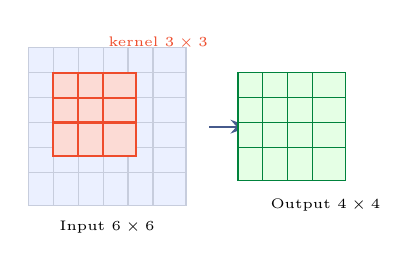
\begin{tikzpicture}[scale=0.72]
  % Input 6x6
  \foreach \i in {0,...,5} \foreach \j in {0,...,5} {
    \node[draw=ptmid!30, fill=ptlight, minimum size=0.42cm]
      at (\j*0.44, -\i*0.44) {};
  }
  \node[below, font=\tiny] at (1.1, -2.6) {Input $6\times6$};

  % Kernel 3x3 highlighted
  \foreach \i in {1,2,3} \foreach \j in {1,2,3} {
    \node[draw=ptred, fill=ptred!20, minimum size=0.42cm, line width=0.8pt]
      at (\j*0.44, -\i*0.44) {};
  }

  \draw[-Stealth, thick, ptmid] (2.9, -1.1) -- (3.6, -1.1);

  % Output 4x4
  \foreach \i in {0,...,3} \foreach \j in {0,...,3} {
    \node[draw=str, fill=green!10, minimum size=0.42cm]
      at (\j*0.44+3.7, -\i*0.44-0.44) {};
  }
  \node[below, font=\tiny] at (4.95, -2.2) {Output $4\times4$};

  % Arrow showing kernel application
  \node[ptred, font=\tiny, above] at (2.0, 0.1) {kernel $3\times3$};
\end{tikzpicture}
\end{center}
\[ \text{out} = \left\lfloor\frac{H+2p-k}{s}\right\rfloor + 1 \]
\end{columns}
\end{frame}

% ─────────────────────────────────────────────────────────────────────────────

\begin{frame}[fragile]{Arquitetura CNN Classica: LeNet-like}
\begin{columns}
\column{0.52\textwidth}
\begin{lstlisting}
class CNN(nn.Module):
    """
    CNN para classificacao de imagens 32x32.
    Segue o padrao: Conv-BN-ReLU-Pool (encoder)
    seguido de MLP (cabeca de classificacao).
    """
    def __init__(self, num_classes: int = 10):
        super().__init__()

        # Extrator de features (encoder)
        self.features = nn.Sequential(
            # Bloco 1: (B,1,32,32) -> (B,32,16,16)
            nn.Conv2d(1, 32, 3, padding=1),
            nn.BatchNorm2d(32), nn.ReLU(),
            nn.MaxPool2d(2),

            # Bloco 2: (B,32,16,16) -> (B,64,8,8)
            nn.Conv2d(32, 64, 3, padding=1),
            nn.BatchNorm2d(64), nn.ReLU(),
            nn.MaxPool2d(2),

            # Bloco 3: (B,64,8,8) -> (B,128,4,4)
            nn.Conv2d(64, 128, 3, padding=1),
            nn.BatchNorm2d(128), nn.ReLU(),
            nn.MaxPool2d(2),
        )
        # Cabeca de classificacao
        self.classifier = nn.Sequential(
            nn.Flatten(),
            nn.Linear(128*4*4, 256),
            nn.ReLU(), nn.Dropout(0.5),
            nn.Linear(256, num_classes),
        )

    def forward(self, x):
        return self.classifier(self.features(x))
\end{lstlisting}

\column{0.46\textwidth}
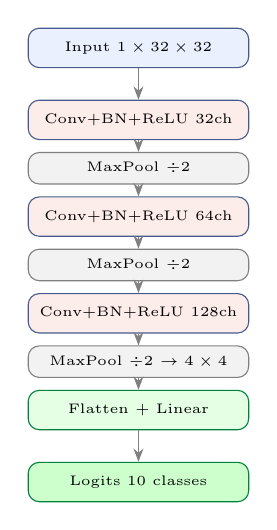
\begin{tikzpicture}[scale=0.75, node distance=0.4cm]
  \node[draw=ptmid, fill=ptlight, rounded corners, minimum width=2.8cm,
        minimum height=0.5cm, text centered, font=\tiny] (inp) {Input $1\times32\times32$};
  \node[draw=ptmid, fill=ptred!10, rounded corners, minimum width=2.8cm,
        minimum height=0.5cm, text centered, font=\tiny, below=of inp] (b1) {Conv+BN+ReLU $32$ch};
  \node[draw=gray, fill=gray!10, rounded corners, minimum width=2.8cm,
        minimum height=0.4cm, text centered, font=\tiny, below=0.15cm of b1] (p1) {MaxPool $\div2$};
  \node[draw=ptmid, fill=ptred!10, rounded corners, minimum width=2.8cm,
        minimum height=0.5cm, text centered, font=\tiny, below=0.15cm of p1] (b2) {Conv+BN+ReLU $64$ch};
  \node[draw=gray, fill=gray!10, rounded corners, minimum width=2.8cm,
        minimum height=0.4cm, text centered, font=\tiny, below=0.15cm of b2] (p2) {MaxPool $\div2$};
  \node[draw=ptmid, fill=ptred!10, rounded corners, minimum width=2.8cm,
        minimum height=0.5cm, text centered, font=\tiny, below=0.15cm of p2] (b3) {Conv+BN+ReLU $128$ch};
  \node[draw=gray, fill=gray!10, rounded corners, minimum width=2.8cm,
        minimum height=0.4cm, text centered, font=\tiny, below=0.15cm of b3] (p3) {MaxPool $\div2$ $\to 4\times4$};
  \node[draw=str, fill=green!10, rounded corners, minimum width=2.8cm,
        minimum height=0.5cm, text centered, font=\tiny, below=0.15cm of p3] (fc) {Flatten + Linear};
  \node[draw=str, fill=green!20, rounded corners, minimum width=2.8cm,
        minimum height=0.5cm, text centered, font=\tiny, below=of fc] (out) {Logits $10$ classes};
  \draw[-Stealth, gray] (inp)--(b1); \draw[-Stealth,gray](b1)--(p1);
  \draw[-Stealth, gray] (p1)--(b2);  \draw[-Stealth,gray](b2)--(p2);
  \draw[-Stealth, gray] (p2)--(b3);  \draw[-Stealth,gray](b3)--(p3);
  \draw[-Stealth, gray] (p3)--(fc);  \draw[-Stealth,gray](fc)--(out);
\end{tikzpicture}
\end{columns}
\end{frame}

% ─────────────────────────────────────────────────────────────────────────────

\begin{frame}[fragile]{Transfer Learning com CNNs Pre-treinadas}
\begin{lstlisting}
import torchvision.models as models

# Carrega ResNet-18 pre-treinada no ImageNet
backbone = models.resnet18(weights='IMAGENET1K_V1')

# Estrategia 1: Feature Extractor
# Congela TODOS os pesos, substitui apenas a cabeca
for param in backbone.parameters():
    param.requires_grad = False

# Substitui a camada final para o numero de classes desejado
backbone.fc = nn.Linear(backbone.fc.in_features, num_classes)
# So a cabeca (fc) sera treinada

# Estrategia 2: Fine-tuning
# Descongela tudo, usa LR menor para as camadas iniciais
for param in backbone.parameters():
    param.requires_grad = True

optimizer = torch.optim.Adam([
    {'params': backbone.layer4.parameters(), 'lr': 1e-4},
    {'params': backbone.fc.parameters(),     'lr': 1e-3},  # LR maior
])

# Modelos disponiveis: resnet18/50/101, efficientnet_b0/b7,
#                      vit_b_16, densenet121, mobilenet_v3_small ...
\end{lstlisting}
\end{frame}

% =============================================================================
\section{Aula 12 — Redes Recorrentes (RNN)}
% =============================================================================

\begin{frame}{Dados Sequenciais e o Problema da Memoria}
\begin{columns}
\column{0.52\textwidth}
\begin{block}{Por que RNNs?}
  MLPs e CNNs assumem que as entradas sao \textbf{independentes}. 
  Em sequencias (texto, audio, series temporais), o contexto passado importa.
  
  \vspace{0.4em}
  A RNN mantem um \textbf{estado oculto} $h_t$ que carrega informacao dos 
  passos anteriores:
  \[
    h_t = f(W_h h_{t-1} + W_x x_t + b)
  \]
  \[
    y_t = W_y h_t + b_y
  \]
\end{block}

\column{0.46\textwidth}
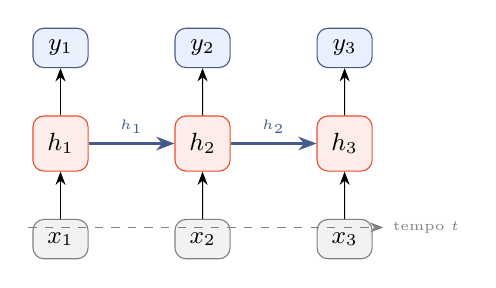
\begin{tikzpicture}[scale=0.82, node distance=0.6cm]
  % Unrolled RNN (3 steps)
  \foreach \t/\xpos in {1/0, 2/2.2, 3/4.4} {
    \node[draw=ptred, fill=ptred!10, rounded corners, minimum size=0.7cm,
          text centered, font=\small] (h\t) at (\xpos, 0) {$h_\t$};
    \node[draw=ptmid, fill=ptlight, rounded corners, minimum width=0.7cm,
          minimum height=0.5cm, font=\small, above=0.6cm of h\t] (y\t) {$y_\t$};
    \node[draw=gray, fill=gray!10, rounded corners, minimum width=0.7cm,
          minimum height=0.5cm, font=\small, below=0.6cm of h\t] (x\t) {$x_\t$};
    \draw[-Stealth] (x\t) -- (h\t);
    \draw[-Stealth] (h\t) -- (y\t);
  }
  % Recurrent connections
  \draw[-Stealth, ptmid, thick] (h1) -- node[above, font=\tiny]{$h_1$}(h2);
  \draw[-Stealth, ptmid, thick] (h2) -- node[above, font=\tiny]{$h_2$}(h3);
  % Time arrow
  \draw[-Stealth, gray, dashed] (-0.5,-1.3) -- (5,-1.3)
    node[right, font=\tiny]{tempo $t$};
\end{tikzpicture}
\end{columns}
\end{frame}

% ─────────────────────────────────────────────────────────────────────────────

\begin{frame}[fragile]{RNN Simples, LSTM e GRU em PyTorch}
\begin{columns}
\column{0.5\textwidth}
\begin{lstlisting}
# RNN simples (problema: vanishing gradient)
rnn = nn.RNN(
    input_size=64,    # dim de cada x_t
    hidden_size=128,  # dim do estado oculto
    num_layers=2,     # RNNs empilhadas
    batch_first=True, # (B, T, F) em vez de (T,B,F)
    dropout=0.3,
)

# LSTM: gates resolvem vanishing gradient
lstm = nn.LSTM(
    input_size=64, hidden_size=128,
    num_layers=2, batch_first=True,
    dropout=0.3, bidirectional=False,
)

# GRU: mais leve que LSTM, desempenho similar
gru = nn.GRU(
    input_size=64, hidden_size=128,
    num_layers=2, batch_first=True,
)
\end{lstlisting}

\column{0.48\textwidth}
\begin{lstlisting}
# Forward pass
x = torch.randn(32, 50, 64)
# x: (batch=32, seq_len=50, input=64)

# RNN/GRU: retorna (output, h_n)
out, h_n = gru(x)
# out: (32, 50, 128) -- todos os h_t
# h_n: (2, 32, 128)  -- ultimo h_t

# LSTM: retorna (output, (h_n, c_n))
out, (h_n, c_n) = lstm(x)
# c_n: cell state (especifico do LSTM)

# Classificacao de sequencia:
# usa apenas o ultimo passo de tempo
ultimo = out[:, -1, :]   # (B, 128)
logits = nn.Linear(128, num_classes)(ultimo)

# Para classificacao com LSTM
# inicializacao do estado oculto:
h0 = torch.zeros(2, 32, 128)
c0 = torch.zeros(2, 32, 128)
out, _ = lstm(x, (h0, c0))
\end{lstlisting}
\end{columns}
\end{frame}

% ─────────────────────────────────────────────────────────────────────────────

\begin{frame}[fragile]{Exemplo Completo: Classificador de Texto com GRU}
\begin{lstlisting}[style=small]
class ClassificadorGRU(nn.Module):
    """
    Classifica sequencias de tokens em num_classes categorias.
    Fluxo: indices de tokens -> embeddings -> GRU -> classificacao
    """
    def __init__(self, vocab_size: int, embed_dim: int,
                 hidden_dim: int, num_classes: int, num_layers: int = 2):
        super().__init__()
        # Embedding: converte indices inteiros em vetores densos
        self.embedding = nn.Embedding(vocab_size, embed_dim,
                                      padding_idx=0)  # 0 = <PAD>
        self.gru = nn.GRU(embed_dim, hidden_dim, num_layers,
                          batch_first=True, dropout=0.3,
                          bidirectional=True)    # bidirecional: le em ambas direcoes
        # *2 porque bidirecional concatena forward + backward
        self.head = nn.Linear(hidden_dim * 2, num_classes)
        self.dropout = nn.Dropout(0.3)

    def forward(self, x: torch.Tensor) -> torch.Tensor:
        # x: (B, T) -- indices de tokens (inteiros)
        emb = self.dropout(self.embedding(x))  # (B, T, embed_dim)
        out, _ = self.gru(emb)                 # (B, T, hidden*2)
        # Usa o ultimo token como representacao da sequencia
        return self.head(self.dropout(out[:, -1, :]))

# Uso
modelo = ClassificadorGRU(vocab_size=10000, embed_dim=128,
                          hidden_dim=256, num_classes=2)
x = torch.randint(0, 10000, (32, 100))  # batch de 32 sequencias de len 100
print(modelo(x).shape)                  # (32, 2)
\end{lstlisting}
\end{frame}

% ─────────────────────────────────────────────────────────────────────────────

\begin{frame}{RNN vs LSTM vs GRU: Quando usar cada uma}
\centering
\begin{tabular}{lccc}
\toprule
& \textbf{RNN} & \textbf{LSTM} & \textbf{GRU} \\
\midrule
Parametros & menos & mais & medio \\
Vanishing gradient & sim & resolvido & resolvido \\
Velocidade de treino & rapida & lenta & media \\
Sequencias longas & ruim & otima & boa \\
\midrule
\textbf{Use quando} & prototipo & dependencias & balanco \\
& rapido & longas & perf/custo \\
\bottomrule
\end{tabular}

\vspace{0.8em}
\begin{destaque}
  \textbf{Atencao:} Em NLP moderno, Transformers (BERT, GPT) superam RNNs em 
  quase todas as tarefas. RNNs ainda sao relevantes para \textbf{series temporais}, 
  \textbf{audio} e cenarios de \textbf{recursos limitados} onde a complexidade 
  quadratica do Transformer e proibitiva.
\end{destaque}
\end{frame}

% =============================================================================
\section{Aula 13 — GANs: Fundamentos}
% =============================================================================

\begin{frame}{O que é uma GAN?}
\begin{columns}
\column{0.55\textwidth}
  \begin{block}{Ideia (Goodfellow et al. 2014)}
    Duas redes em \textbf{jogo adversarial}:
    \begin{itemize}
      \item \textbf{Gerador} $G$: transforma ruído $z \sim p_z$ em dados falsos
      \item \textbf{Discriminador} $D$: distingue dados reais de falsos
    \end{itemize}
    
    $G$ tenta enganar $D$; $D$ tenta não ser enganado.
  \end{block}
  
  \vspace{0.4em}
  \textbf{Objetivo (minimax):}
  \[
    \min_G \max_D \; \E_{x \sim p_\text{data}}[\log D(x)] + \E_{z \sim p_z}[\log(1 - D(G(z)))]
  \]

\column{0.42\textwidth}
  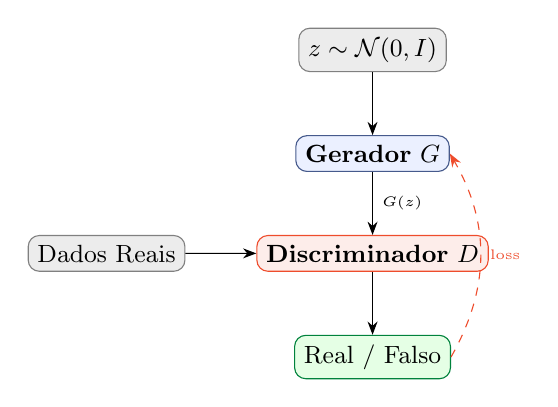
\begin{tikzpicture}[scale=0.85, node distance=0.8cm]
    \node[draw=gray, fill=gray!15, rounded corners, minimum width=1.8cm,
          text centered, font=\small] (z) {$z \sim \mathcal{N}(0,I)$};
    \node[draw=ptmid, fill=ptlight, rounded corners, minimum width=1.8cm,
          text centered, font=\small, below=of z] (G) {\textbf{Gerador} $G$};
    \node[draw=ptred, fill=ptred!10, rounded corners, minimum width=1.8cm,
          text centered, font=\small, below=of G] (D) {\textbf{Discriminador} $D$};
    \node[draw=gray, fill=gray!15, rounded corners, minimum width=1.8cm,
          text centered, font=\small, left=0.9cm of D] (real) {Dados Reais};
    \node[draw=str, fill=green!10, rounded corners, minimum width=1.8cm,
          text centered, font=\small, below=of D] (out) {Real / Falso};
    \draw[-Stealth] (z) -- (G);
    \draw[-Stealth] (G) -- node[right, font=\tiny]{$G(z)$} (D);
    \draw[-Stealth] (real) -- (D);
    \draw[-Stealth] (D) -- (out);
    \draw[-Stealth, ptred, dashed, bend right] (out.east) to
      node[right, font=\tiny]{\color{ptred}loss} (G.east);
  \end{tikzpicture}
\end{columns}
\end{frame}

% ─────────────────────────────────────────────────────────────────────────────

\begin{frame}[fragile]{Gerador e Discriminador — MLP simples}
\begin{lstlisting}
# Gerador: ruido z -> imagem falsa
class Gerador(nn.Module):
    def __init__(self, z_dim=100, img_dim=784):  # 784 = 28*28 (MNIST)
        super().__init__()
        self.net = nn.Sequential(
            nn.Linear(z_dim, 256),
            nn.LeakyReLU(0.2),
            nn.Linear(256, 512),
            nn.LeakyReLU(0.2),
            nn.Linear(512, img_dim),
            nn.Tanh(),         # output em [-1, 1]
        )
    def forward(self, z):
        return self.net(z)

# Discriminador: imagem -> probabilidade de ser real
class Discriminador(nn.Module):
    def __init__(self, img_dim=784):
        super().__init__()
        self.net = nn.Sequential(
            nn.Linear(img_dim, 512),
            nn.LeakyReLU(0.2),
            nn.Linear(512, 256),
            nn.LeakyReLU(0.2),
            nn.Linear(256, 1),
            # SEM Sigmoid aqui -- BCEWithLogitsLoss ja aplica
        )
    def forward(self, x):
        return self.net(x)
\end{lstlisting}
\end{frame}

% ─────────────────────────────────────────────────────────────────────────────

\begin{frame}[fragile]{Loop de Treino da GAN}
\begin{lstlisting}[style=small]
G = Gerador(z_dim=100).to(device)
D = Discriminador().to(device)
opt_G = optim.Adam(G.parameters(), lr=2e-4, betas=(0.5, 0.999))
opt_D = optim.Adam(D.parameters(), lr=2e-4, betas=(0.5, 0.999))
criterio = nn.BCEWithLogitsLoss()

for epoch in range(n_epochs):
    for x_real, _ in loader:
        x_real = x_real.view(-1, 784).to(device)  # achata para MLP
        B = x_real.size(0)

        # ── TREINO DO DISCRIMINADOR ───────────────────────────────
        z       = torch.randn(B, 100, device=device)
        x_falso = G(z).detach()   # .detach(): nao propaga para G!

        pred_real  = D(x_real)
        pred_falso = D(x_falso)
        loss_D = criterio(pred_real,  torch.ones_like(pred_real)) + \
                 criterio(pred_falso, torch.zeros_like(pred_falso))

        opt_D.zero_grad(); loss_D.backward(); opt_D.step()

        # ── TREINO DO GERADOR ─────────────────────────────────────
        z       = torch.randn(B, 100, device=device)
        x_falso = G(z)             # SEM .detach() -- precisamos do gradiente
        pred    = D(x_falso)
        # G quer que D classifique seus outputs como "real" (label=1)
        loss_G  = criterio(pred, torch.ones_like(pred))

        opt_G.zero_grad(); loss_G.backward(); opt_G.step()
\end{lstlisting}
\end{frame}

% ─────────────────────────────────────────────────────────────────────────────

\begin{frame}{O Detalhe Crucial: \texttt{.detach()}}
\begin{columns}
\column{0.5\textwidth}
\begin{block}{Treino do Discriminador}
  Queremos atualizar \textbf{apenas} $D$.\\
  Se não usarmos \texttt{.detach()}, o grafo computacional conecta $D$ a $G$, 
  e gradientes fluiriam para $G$ indevidamente.
  
  \vspace{0.3em}
  \texttt{x\_falso = G(z).detach()}\\
  cria uma cópia sem histórico — $D$ vê apenas o tensor, sem saber que veio de $G$.
\end{block}

\column{0.48\textwidth}
\begin{alertblock}{Treino do Gerador}
  Queremos atualizar \textbf{apenas} $G$ através de $D$.\\
  \textbf{Não} use \texttt{.detach()} aqui — o gradiente precisa percorrer:
  \[ D(G(z)) \xrightarrow{\text{backward}} G \]
  
  Por isso usamos dois otimizadores separados e zeramos gradientes independentemente.
\end{alertblock}
\end{columns}
\end{frame}

% =============================================================================
\section{Aula 14 — DCGAN e Boas Praticas}
% =============================================================================

\begin{frame}[fragile]{DCGAN: GAN com Convoluções}
\begin{lstlisting}[style=small]
# Gerador DCGAN (z -> imagem 64x64)
class GeradorDC(nn.Module):
    def __init__(self, z_dim=100, ngf=64):
        super().__init__()
        self.net = nn.Sequential(
            # z: (B, 100, 1, 1) -> (B, ngf*8, 4, 4)
            nn.ConvTranspose2d(z_dim, ngf*8, 4, 1, 0, bias=False),
            nn.BatchNorm2d(ngf*8), nn.ReLU(),
            # (B, ngf*8, 4, 4) -> (B, ngf*4, 8, 8)
            nn.ConvTranspose2d(ngf*8, ngf*4, 4, 2, 1, bias=False),
            nn.BatchNorm2d(ngf*4), nn.ReLU(),
            # -> (B, ngf*2, 16, 16)
            nn.ConvTranspose2d(ngf*4, ngf*2, 4, 2, 1, bias=False),
            nn.BatchNorm2d(ngf*2), nn.ReLU(),
            # -> (B, ngf, 32, 32)
            nn.ConvTranspose2d(ngf*2, ngf, 4, 2, 1, bias=False),
            nn.BatchNorm2d(ngf), nn.ReLU(),
            # -> (B, 3, 64, 64)
            nn.ConvTranspose2d(ngf, 3, 4, 2, 1, bias=False),
            nn.Tanh(),
        )
    def forward(self, z):
        return self.net(z.view(z.size(0), -1, 1, 1))
\end{lstlisting}
\end{frame}

% ─────────────────────────────────────────────────────────────────────────────

\begin{frame}[fragile]{Discriminador DCGAN}
\begin{lstlisting}
class DiscriminadorDC(nn.Module):
    def __init__(self, ndf=64):
        super().__init__()
        self.net = nn.Sequential(
            # (B, 3, 64, 64) -> (B, ndf, 32, 32)
            nn.Conv2d(3, ndf, 4, 2, 1, bias=False),
            nn.LeakyReLU(0.2),
            # -> (B, ndf*2, 16, 16)
            nn.Conv2d(ndf, ndf*2, 4, 2, 1, bias=False),
            nn.BatchNorm2d(ndf*2), nn.LeakyReLU(0.2),
            # -> (B, ndf*4, 8, 8)
            nn.Conv2d(ndf*2, ndf*4, 4, 2, 1, bias=False),
            nn.BatchNorm2d(ndf*4), nn.LeakyReLU(0.2),
            # -> (B, ndf*8, 4, 4)
            nn.Conv2d(ndf*4, ndf*8, 4, 2, 1, bias=False),
            nn.BatchNorm2d(ndf*8), nn.LeakyReLU(0.2),
            # -> (B, 1, 1, 1)
            nn.Conv2d(ndf*8, 1, 4, 1, 0, bias=False),
        )
    def forward(self, x):
        return self.net(x).view(-1, 1)  # achata para (B, 1)
\end{lstlisting}
\end{frame}

% ─────────────────────────────────────────────────────────────────────────────

\begin{frame}[fragile]{Inicialização de Pesos}
\begin{lstlisting}
# DCGAN recomenda: N(0, 0.02) para Conv e ConvTranspose
#                 N(1, 0.02) + bias=0 para BatchNorm
def inicializar_pesos(m):
    classname = m.__class__.__name__
    if 'Conv' in classname:
        nn.init.normal_(m.weight.data, 0.0, 0.02)
    elif 'BatchNorm' in classname:
        nn.init.normal_(m.weight.data, 1.0, 0.02)
        nn.init.constant_(m.bias.data, 0)

G = GeradorDC().to(device)
D = DiscriminadorDC().to(device)

G.apply(inicializar_pesos)  # aplica recursivamente a todos os submodulos
D.apply(inicializar_pesos)
\end{lstlisting}

\begin{block}{\texttt{.apply(fn)}}
  Percorre recursivamente todos os sub-modulos e aplica \texttt{fn} a cada um.
  Essencial para inicializacoes customizadas.
\end{block}
\end{frame}

% ─────────────────────────────────────────────────────────────────────────────

\begin{frame}{Boas Praticas para GANs}
\begin{columns}
\column{0.5\textwidth}
\begin{block}{\faCheck\ Faca}
  \begin{itemize}
    \item Use \texttt{LeakyReLU(0.2)} no discriminador
    \item Use \texttt{Tanh} no output do gerador
    \item Normalize dados para $[-1, 1]$
    \item Dois otimizadores separados (G e D)
    \item \texttt{bias=False} com BatchNorm
    \item Inicialize pesos com $\mathcal{N}(0, 0.02)$
    \item Adam com $\beta_1=0.5$
  \end{itemize}
\end{block}

\column{0.48\textwidth}
\begin{alertblock}{\faTimes\ Evite}
  \begin{itemize}
    \item Treinar D muito mais que G (ou vice-versa)
    \item Usar BatchNorm no input do D
    \item Usar BatchNorm no output do G
    \item Learning rate alto ($> 5 \times 10^{-4}$)
    \item Batch size muito pequeno ($< 32$)
  \end{itemize}
\end{alertblock}
\end{columns}

\vspace{0.4em}
\begin{destaque}
  \textbf{Mode collapse} (o gerador produz sempre a mesma saida) e o problema mais comum. 
  Sinal: \texttt{loss\_D} cai para zero, \texttt{loss\_G} explode.
\end{destaque}
\end{frame}

% =============================================================================
\section{Aula 15 — Reinforcement Learning}
% =============================================================================

\begin{frame}{O Paradigma do Aprendizado por Reforco}
\begin{columns}
\column{0.52\textwidth}
\begin{block}{Definicao}
  Um \textbf{agente} interage com um \textbf{ambiente} tomando \textbf{acoes},
  observando \textbf{estados} e recebendo \textbf{recompensas}. 
  O objetivo e aprender uma \textbf{politica} $\pi(a|s)$ que maximiza 
  a recompensa acumulada futura:
  \[
    G_t = \sum_{k=0}^{\infty} \gamma^k r_{t+k}
  \]
  $\gamma \in (0,1]$: fator de desconto (valoriza recompensas proximas).
\end{block}
\vspace{0.3em}
\textbf{Diferenca dos outros paradigmas:}
\begin{itemize}
  \item Sem rotulos supervisionados
  \item Feedback esparso e atrasado (credito temporal)
  \item Agente influencia os proprios dados que coleta
\end{itemize}

\column{0.46\textwidth}
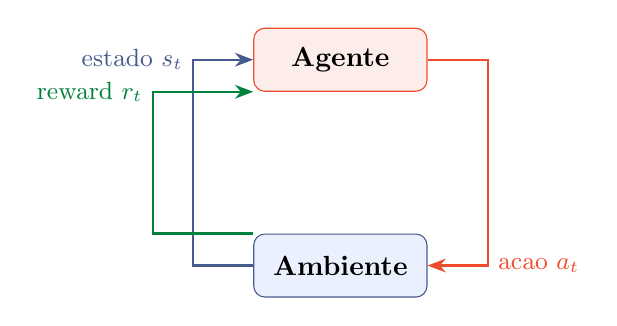
\begin{tikzpicture}[scale=0.85, node distance=0.9cm]
  \node[draw=ptred, fill=ptred!10, rounded corners,
        minimum width=2.2cm, minimum height=0.8cm,
        text centered] (agente) {\textbf{Agente}};
  \node[draw=ptmid, fill=ptlight, rounded corners,
        minimum width=2.2cm, minimum height=0.8cm,
        text centered, below=1.8cm of agente] (env) {\textbf{Ambiente}};
  \draw[-Stealth, thick, ptred]
    (agente.east) -- ++(0.9,0) |- (env.east)
    node[midway, right, font=\small]{acao $a_t$};
  \draw[-Stealth, thick, ptmid]
    (env.west) -- ++(-0.9,0) |- (agente.west)
    node[midway, left, font=\small]{estado $s_t$};
  \draw[-Stealth, thick, str]
    (env.north west) -- ++(-1.5,0) |- (agente.south west)
    node[midway, left, font=\small, str]{reward $r_t$};
\end{tikzpicture}
\end{columns}
\end{frame}

% ─────────────────────────────────────────────────────────────────────────────

\begin{frame}{Conceitos Fundamentais}
\begin{columns}
\column{0.5\textwidth}
\begin{block}{Funcao Valor $V^\pi(s)$}
  Recompensa acumulada esperada a partir do estado $s$ seguindo $\pi$:
  \[
    V^\pi(s) = \mathbb{E}_\pi\!\left[G_t \mid s_t = s\right]
  \]
\end{block}
\begin{block}{Funcao Q $Q^\pi(s,a)$}
  Recompensa acumulada esperada tomando acao $a$ em $s$, depois seguindo $\pi$:
  \[
    Q^\pi(s,a) = \mathbb{E}_\pi\!\left[G_t \mid s_t = s, a_t = a\right]
  \]
  \textbf{Politica otima:} $\pi^*(s) = \arg\max_a Q^*(s,a)$
\end{block}

\column{0.48\textwidth}
\begin{block}{Equacao de Bellman}
  \[
    Q(s,a) = r + \gamma \max_{a'} Q(s', a')
  \]
  Relaciona o valor atual com o valor do proximo estado. 
  Base de todos os algoritmos de Q-learning.
\end{block}
\begin{block}{Algoritmos principais}
  \begin{itemize}
    \item \textbf{DQN}: Q-learning com rede neural
    \item \textbf{PPO}: Policy gradient com clipping
    \item \textbf{A3C}: Actor-Critic assincronico
    \item \textbf{SAC}: Maximo de entropia (continuo)
  \end{itemize}
\end{block}
\end{columns}
\end{frame}

% ─────────────────────────────────────────────────────────────────────────────

\begin{frame}[fragile]{DQN: Deep Q-Network}
\begin{columns}
\column{0.52\textwidth}
\begin{lstlisting}
class DQN(nn.Module):
    """
    Rede Q: mapeia estado -> Q-valor de cada acao.
    Para o CartPole: estado (4,), acoes (2,)
    """
    def __init__(self, state_dim: int,
                 n_actions: int):
        super().__init__()
        self.net = nn.Sequential(
            nn.Linear(state_dim, 128),
            nn.ReLU(),
            nn.Linear(128, 128),
            nn.ReLU(),
            nn.Linear(128, n_actions),
        )

    def forward(self, s: torch.Tensor):
        return self.net(s)
        # retorna Q(s, a) para cada acao

# Politica epsilon-greedy
def escolher_acao(model, estado, epsilon):
    if torch.rand(1).item() < epsilon:
        return torch.randint(n_actions, (1,)).item()
    with torch.no_grad():
        q_vals = model(torch.tensor(estado))
        return q_vals.argmax().item()
\end{lstlisting}

\column{0.46\textwidth}
\begin{block}{Replay Buffer}
  O DQN usa um buffer para armazenar transicoes $(s, a, r, s', done)$ 
  e amostrar mini-batches. Isso quebra correlacao entre amostras consecutivas.
\end{block}
\begin{lstlisting}[basicstyle=\ttfamily\tiny]
from collections import deque
import random

class ReplayBuffer:
    def __init__(self, capacity=10000):
        self.buffer = deque(maxlen=capacity)

    def push(self, s, a, r, s_, done):
        self.buffer.append((s,a,r,s_,done))

    def sample(self, batch_size):
        batch = random.sample(
            self.buffer, batch_size)
        s,a,r,s_,d = zip(*batch)
        return (torch.tensor(s,  dtype=torch.float32),
                torch.tensor(a),
                torch.tensor(r,  dtype=torch.float32),
                torch.tensor(s_, dtype=torch.float32),
                torch.tensor(d,  dtype=torch.float32))

    def __len__(self):
        return len(self.buffer)
\end{lstlisting}
\end{columns}
\end{frame}

% ─────────────────────────────────────────────────────────────────────────────

\begin{frame}[fragile]{Loop de Treino do DQN}
\begin{lstlisting}[style=small]
import gymnasium as gym  # pip install gymnasium

env = gym.make('CartPole-v1')  # estado: (4,), acoes: {0, 1}

modelo     = DQN(state_dim=4, n_actions=2).to(device)
target_net = DQN(state_dim=4, n_actions=2).to(device)
target_net.load_state_dict(modelo.state_dict())   # copia inicial

buffer    = ReplayBuffer(capacity=10000)
opt       = torch.optim.Adam(modelo.parameters(), lr=1e-4)
crit      = nn.MSELoss()
epsilon   = 1.0    # exploracao inicial: 100%
gamma     = 0.99

for episodio in range(500):
    estado, _ = env.reset()
    for passo in range(500):
        acao  = escolher_acao(modelo, estado, epsilon)
        prox, reward, done, trunc, _ = env.step(acao)
        buffer.push(estado, acao, reward, prox, done or trunc)
        estado = prox

        if len(buffer) >= 512:
            s, a, r, s_, d = [t.to(device) for t in buffer.sample(64)]
            q_atual  = modelo(s).gather(1, a.unsqueeze(1)).squeeze()
            q_target = r + gamma * target_net(s_).max(1).values * (1 - d)
            loss = crit(q_atual, q_target.detach())   # .detach(): target fixo!
            opt.zero_grad(); loss.backward(); opt.step()

        if done or trunc: break

    epsilon = max(0.01, epsilon * 0.995)             # decai epsilon
    if episodio % 10 == 0:                           # atualiza rede target
        target_net.load_state_dict(modelo.state_dict())
\end{lstlisting}
\end{frame}

% ─────────────────────────────────────────────────────────────────────────────

\begin{frame}[fragile]{REINFORCE: Policy Gradient Simples}
\begin{columns}
\column{0.5\textwidth}
\begin{block}{Ideia}
  Em vez de aprender $Q(s,a)$, otimiza diretamente a politica $\pi_\theta(a|s)$.
  O gradiente da politica e:
  \[
    \nabla_\theta J \propto \mathbb{E}\!\left[G_t \nabla_\theta \log \pi_\theta(a_t|s_t)\right]
  \]
  Acoes que levaram a alta recompensa tem sua probabilidade \textbf{aumentada}.
\end{block}

\begin{lstlisting}[basicstyle=\ttfamily\tiny]
class PolicyNet(nn.Module):
    def __init__(self, state_dim, n_actions):
        super().__init__()
        self.net = nn.Sequential(
            nn.Linear(state_dim, 128), nn.ReLU(),
            nn.Linear(128, n_actions),
        )
    def forward(self, s):
        return torch.softmax(self.net(s), dim=-1)
\end{lstlisting}

\column{0.48\textwidth}
\begin{lstlisting}
def treinar_episodio(env, policy, opt):
    estados, acoes, rewards = [], [], []
    s, _ = env.reset()
    done = False

    while not done:
        probs = policy(torch.tensor(s))
        dist  = torch.distributions.Categorical(probs)
        a     = dist.sample()          # amostra acao
        s, r, done, trunc, _ = env.step(a.item())
        estados.append(s); acoes.append(a)
        rewards.append(r)
        done = done or trunc

    # Retornos descontados
    G, retornos = 0, []
    for r in reversed(rewards):
        G = r + 0.99 * G
        retornos.insert(0, G)
    R = torch.tensor(retornos)
    R = (R - R.mean()) / (R.std() + 1e-8)  # baseline

    # Loss: -log_prob * retorno
    loss = 0
    for s, a, g in zip(estados, acoes, R):
        p = policy(torch.tensor(s))
        d = torch.distributions.Categorical(p)
        loss -= d.log_prob(a) * g    # gradiente de politica

    opt.zero_grad(); loss.backward(); opt.step()
\end{lstlisting}
\end{columns}
\end{frame}

% ─────────────────────────────────────────────────────────────────────────────

\begin{frame}{RL no PyTorch: Resumo dos Componentes}
\centering
\begin{tabular}{lll}
\toprule
\textbf{Componente} & \textbf{O que e} & \textbf{PyTorch} \\
\midrule
Politica $\pi_\theta(a|s)$ & Rede que decide acoes & \texttt{nn.Module} \\
Funcao Q $Q_\theta(s,a)$ & Rede que estima valores & \texttt{nn.Module} \\
Replay Buffer & Armazena transicoes & \texttt{deque} / \texttt{Tensor} \\
Target Network & Copia estavel da Q-net & \texttt{load\_state\_dict} \\
Distribuicao de acao & Amostragem diferenciavel & \texttt{torch.distributions} \\
Loss de valor & Bellman residual & \texttt{nn.MSELoss} \\
Loss de politica & $-\log\pi \cdot G$ & calculo manual \\
\bottomrule
\end{tabular}
\vspace{0.6em}
\begin{destaque}
  Para RL em producao, use bibliotecas especializadas: 
  \textbf{Stable-Baselines3} (PyTorch), \textbf{RLlib}, ou \textbf{CleanRL}.
  Elas ja implementam DQN, PPO, SAC com hiperparametros validados.
\end{destaque}
\end{frame}

% =============================================================================
\section{Aula 16 — Diagnostico e Ferramentas}
% =============================================================================

\begin{frame}[fragile]{Monitorando o Treino com TensorBoard}
\begin{lstlisting}
from torch.utils.tensorboard import SummaryWriter

writer = SummaryWriter('runs/experimento_01')

for epoch in range(n_epochs):
    # ... loop de treino ...

    # Escalares
    writer.add_scalar('Loss/Gerador',       loss_G.item(), epoch)
    writer.add_scalar('Loss/Discriminador', loss_D.item(), epoch)

    # Imagens geradas
    with torch.no_grad():
        z = torch.randn(64, 100, device=device)
        amostras = G(z).reshape(-1, 1, 28, 28) * 0.5 + 0.5
        writer.add_images('Amostras/Geradas', amostras, epoch)

    # Histograma de pesos
    for nome, param in G.named_parameters():
        writer.add_histogram(f'G/{nome}', param, epoch)

writer.close()
\end{lstlisting}

\begin{lstlisting}[style=bash]
tensorboard --logdir=runs    # abre no navegador: http://localhost:6006
\end{lstlisting}
\end{frame}

% ─────────────────────────────────────────────────────────────────────────────

\begin{frame}[fragile]{Depurando Problemas Comuns}
\begin{columns}
\column{0.52\textwidth}
\begin{alertblock}{Gradientes explodindo}
\begin{lstlisting}[numbers=none]
# Sintoma: loss = nan, inf
# Solucao: gradient clipping
nn.utils.clip_grad_norm_(
    model.parameters(),
    max_norm=1.0
)
# Sempre ANTES do optimizer.step()
\end{lstlisting}
\end{alertblock}

\begin{alertblock}{Tensores em devices errados}
\begin{lstlisting}[numbers=none]
# RuntimeError: Expected all tensors
# to be on the same device
# Solucao: mova tudo para device
x = x.to(device)
y = y.to(device)
model = model.to(device)
\end{lstlisting}
\end{alertblock}

\column{0.46\textwidth}
\begin{alertblock}{Sem memoria (OOM)}
\begin{lstlisting}[numbers=none]
# CUDA out of memory
# 1. Reduza batch_size
# 2. Use no_grad na validacao
# 3. Libere cache
torch.cuda.empty_cache()
# 4. Acumule gradientes
loss = loss / n_acc
loss.backward()
if step % n_acc == 0:
    optimizer.step()
    optimizer.zero_grad()
\end{lstlisting}
\end{alertblock}

\begin{exampleblock}{Verifica shapes}
\begin{lstlisting}[numbers=none]
# Adicione prints no forward:
def forward(self, x):
    print(x.shape)   # debug!
    x = self.conv(x)
    print(x.shape)
    return x
\end{lstlisting}
\end{exampleblock}
\end{columns}
\end{frame}

% ─────────────────────────────────────────────────────────────────────────────

\begin{frame}[fragile]{Precisao Mista (Automatic Mixed Precision)}
\begin{lstlisting}
from torch.cuda.amp import autocast, GradScaler

scaler = GradScaler()

for x, y in loader:
    x, y = x.to(device), y.to(device)

    # autocast: usa float16 onde e seguro, float32 onde necessario
    with autocast():
        pred = model(x)
        loss = criterio(pred, y)

    optimizer.zero_grad()

    # scaler: evita underflow de gradientes em float16
    scaler.scale(loss).backward()
    scaler.step(optimizer)
    scaler.update()
\end{lstlisting}

\begin{block}{Benefícios da Precisão Mista}
  \begin{itemize}
    \item $\approx 2\times$ mais rápido em GPUs com Tensor Cores (Ampere, Ada)
    \item Reduz uso de VRAM pela metade para os activations
    \item Permite batches maiores
  \end{itemize}
\end{block}
\end{frame}

% =============================================================================
\section{Referência Rápida}
% =============================================================================

\begin{frame}{Mapa Conceitual Completo}
\begin{center}
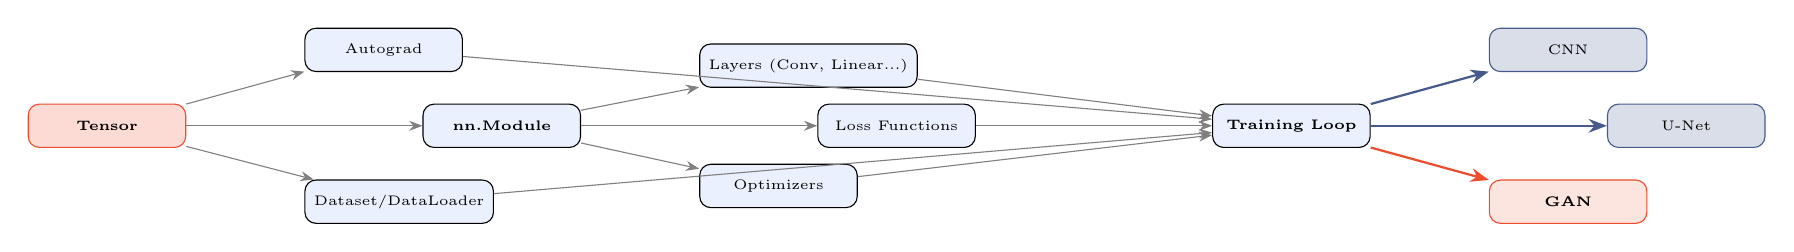
\begin{tikzpicture}[scale=0.78, node distance=0.6cm,
  box/.style={draw, rounded corners, fill=ptlight, minimum width=2cm,
              minimum height=0.55cm, text centered, font=\tiny}]

  \node[box, fill=ptred!20, draw=ptred] (tensor) {\textbf{Tensor}};

  \node[box, above right=0.4cm and 1.5cm of tensor] (autograd) {Autograd};
  \node[box, right=3cm of tensor] (module) {\textbf{nn.Module}};
  \node[box, below right=0.4cm and 1.5cm of tensor] (data) {Dataset/DataLoader};

  \node[box, above right=0.2cm and 1.5cm of module] (layers) {Layers (Conv, Linear...)};
  \node[box, right=3cm of module] (loss) {Loss Functions};
  \node[box, below right=0.2cm and 1.5cm of module] (optim) {Optimizers};

  \node[box, right=3cm of loss] (loop) {\textbf{Training Loop}};

  \node[box, above right=0.4cm and 1.5cm of loop, fill=ptmid!20, draw=ptmid] (cnn) {CNN};
  \node[box, right=3cm of loop, fill=ptmid!20, draw=ptmid] (unet) {U-Net};
  \node[box, below right=0.4cm and 1.5cm of loop, fill=ptred!15, draw=ptred] (gan) {\textbf{GAN}};

  \draw[-Stealth, gray] (tensor) -- (autograd);
  \draw[-Stealth, gray] (tensor) -- (module);
  \draw[-Stealth, gray] (tensor) -- (data);
  \draw[-Stealth, gray] (autograd) -- (loop);
  \draw[-Stealth, gray] (module) -- (layers);
  \draw[-Stealth, gray] (module) -- (loss);
  \draw[-Stealth, gray] (module) -- (optim);
  \draw[-Stealth, gray] (layers) -- (loop);
  \draw[-Stealth, gray] (loss) -- (loop);
  \draw[-Stealth, gray] (optim) -- (loop);
  \draw[-Stealth, gray] (data) -- (loop);
  \draw[-Stealth, ptmid, thick] (loop) -- (cnn);
  \draw[-Stealth, ptmid, thick] (loop) -- (unet);
  \draw[-Stealth, ptred, thick] (loop) -- (gan);
\end{tikzpicture}
\end{center}
\end{frame}

% ─────────────────────────────────────────────────────────────────────────────

\begin{frame}{Tabela de Referência: Camadas}
\centering
\small
\begin{tabular}{lll}
\toprule
\textbf{Camada} & \textbf{Input} & \textbf{Uso típico} \\
\midrule
\texttt{nn.Linear(in, out)} & $(B, in)$ & MLP, head \\
\texttt{nn.Conv2d(in, out, k)} & $(B, in, H, W)$ & Feature extraction \\
\texttt{nn.ConvTranspose2d} & $(B, in, H, W)$ & Upsampling (GAN, U-Net) \\
\texttt{nn.BatchNorm2d(C)} & $(B, C, H, W)$ & Estabilizar treino \\
\texttt{nn.GroupNorm(G, C)} & $(B, C, H, W)$ & Batch size pequeno \\
\texttt{nn.MaxPool2d(2)} & $(B, C, H, W)$ & Downsampling \\
\texttt{nn.Upsample(2)} & $(B, C, H, W)$ & Upsampling suave \\
\texttt{nn.Dropout(p)} & qualquer & Regularização \\
\texttt{nn.Embedding(V, D)} & $(B, L)$ int & NLP, tokens \\
\bottomrule
\end{tabular}
\end{frame}

% ─────────────────────────────────────────────────────────────────────────────

\begin{frame}{Tabela de Referência: Os 5 Passos}
\centering
\begin{tabular}{cll}
\toprule
\textbf{Passo} & \textbf{Código} & \textbf{O que acontece} \\
\midrule
1 & \texttt{pred = model(x)} & Forward pass, constrói grafo \\
2 & \texttt{loss = crit(pred, y)} & Calcula escalar da loss \\
3 & \texttt{optimizer.zero\_grad()} & Zera gradientes acumulados \\
4 & \texttt{loss.backward()} & Backprop, preenche \texttt{.grad} \\
5 & \texttt{optimizer.step()} & Atualiza $\theta \leftarrow \theta - \alpha \nabla$ \\
\bottomrule
\end{tabular}

\vspace{1em}
\begin{destaque}
  Este ciclo de 5 passos é a base de \textbf{todo} treinamento em PyTorch — 
  de uma regressão linear a uma GAN com 100M de parâmetros.
  A diferença está apenas na complexidade do modelo e na lógica em torno do loop.
\end{destaque}
\end{frame}

% ─────────────────────────────────────────────────────────────────────────────

\begin{frame}[plain]
\begin{center}
  \vspace{1.5cm}
  {\LARGE \textbf{Fim da Série}}
  
  \vspace{0.5cm}
  {\large Do Tensor à GAN}
  
  \vspace{1.5cm}
  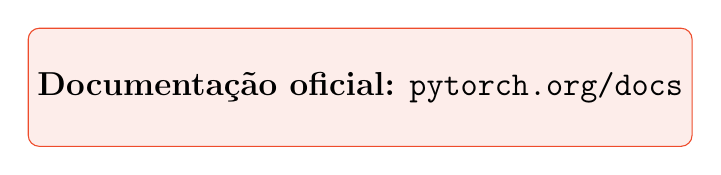
\begin{tikzpicture}
    \node[draw=ptred, fill=ptred!10, rounded corners, minimum width=8cm,
          minimum height=1.5cm, text centered, font=\large] {
      \textbf{Documentação oficial:} \texttt{pytorch.org/docs}
    };
  \end{tikzpicture}
  
  \vspace{1cm}
  {\small
    \begin{tabular}{ccc}
      \texttt{pytorch.org/tutorials} & $\cdot$ &
      \texttt{github.com/pytorch/examples}
    \end{tabular}
  }
\end{center}
\end{frame}

\end{document}
